
\documentclass[a4paper,12pt]{article} % тип документа
%\usepackage{jmlda}

% Рисунки
\usepackage{graphicx}
%\usepackage{epstopdf} %converting to PDF
\usepackage{wrapfig}
\usepackage{multicol}
\graphicspath{ {./images/} }

\usepackage{hyperref}
\hypersetup{				% Гиперссылки
    colorlinks=true,       	% false: ссылки в рамках
    linkcolor=black,
    citecolor=black,
	urlcolor=black          % на URL
}


%  Русский язык

\usepackage[T2A]{fontenc}			% кодировка
\usepackage[utf8]{inputenc}			% кодировка исходного текста
\usepackage[english,russian]{babel}	% локализация и переносы

%отступы слева спраава  сверху снизу
%\oddsidemargin = 5mm
%\textwidth = 165mm
%\topmargin = 0mm
%\voffset = 0mm
%\headsep = 0mm
%\headheight = 0mm
%\textheight = 257mm
\usepackage[left=30mm, top=20mm, right=15mm, bottom=20mm, nohead, footskip=10mm]{geometry} % настройки полей документа
\parindent = 12.5mm%отступ абзаца
\linespread{1.3}%интервал

% Математика
\usepackage{amsmath,amsfonts,amssymb,amsthm,mathtools} 
\usepackage{ dsfont }

\usepackage{color} %% это для отображения цвета в коде
\usepackage{listings} %% собственно, это и есть пакет listings

\usepackage{caption}
\DeclareCaptionFont{white}{\color{white}} %% это сделает текст заголовка белым

\definecolor{dkgreen}{rgb}{0,0.6,0}
\definecolor{gray}{rgb}{0.5,0.5,0.5}
\definecolor{mauve}{rgb}{0.58,0,0.82}

\lstset{ %
language=Python,                 % выбор языка для подсветки (здесь это С)
basicstyle=\small\ttfamily, % размер и начертание шрифта для подсветки кода
numbers=left,               % где поставить нумерацию строк (слева\справа)
numberstyle=\tiny\color{gray},     % Стиль который будет использоваться для нумерации строк
stepnumber=1,                   % размер шага между двумя номерами строк
numbersep=5pt,                % как далеко отстоят номера строк от подсвечиваемого кода
backgroundcolor=\color{white}, % цвет фона подсветки - используем \usepackage{color}
showspaces=false,            % показывать или нет пробелы специальными отступами
showstringspaces=false,      % показывать или нет пробелы в строках
showtabs=false,             % показывать или нет табуляцию в строках
frame=single,              % рисовать рамку вокруг кода
tabsize=2,                 % размер табуляции по умолчанию равен 2 пробелам
captionpos=t,              % позиция заголовка вверху [t] или внизу [b] 
breaklines=true,           % автоматически переносить строки (да\нет)
breakatwhitespace=false, % переносить строки только если есть пробел
escapeinside={\%*}{*)},   % если нужно добавить комментарии в коде
keywordstyle=\color{blue},          % Стиль ключевых слов
commentstyle=\color{dkgreen},       % Стиль комментариев
stringstyle=\color{mauve}\ttfamily,          % Стиль литералов
rulecolor=\color{black},        
title=\lstname,                   % Показать название подгружаемого файла
}


\usepackage{wasysym}

%Заговолок
\author{Хромов~А.\,А.\,~техник 1 категории}
\title{Метод снижения ошибки определения траектории сверхзвукового объекта с помощью рекуррентной нейронной сети, использующей фильтр Калмана}
\date{\today}

%\NOREVIEWERNOTES
\begin{document}
\begin{titlepage}
% НАЧАЛО ТИТУЛЬНОГО ЛИСТА
\begin{center}
\hfill \break
\normalsize{Министерство образования и науки Российской Федерации}\\
\normalsize{Федеральное государственное автономное образовательное учреждение}\\ 
\normalsize{высшего образования}\\
\normalsize{<<Московский физико-технический институт>>\\(национальный исследовательский университет)}\\
\normalsize{Физтех-школа Радиотехники и Компьютерных Технологий}\\
\normalsize{Кафедра радиолокации, управления и информатики}\\
\end{center}
\begin{flushleft}
\normalsize{\textbf{Направление подготовки:} 03.03.01 Прикладные математика и физика}\\
\normalsize{\textbf{Направленность (профиль) подготовки:} Радиотехника и компьютерные технологии}\\
\end{flushleft}
\begin{center}
\hfill\break
\hfill \break
\hfill \break
\hfill \break
\large{\textbf{Метод снижения ошибки определения траектории сверхзвукового объекта с помощью рекуррентной нейронной сети, использующей фильтр Калмана}}\\
\normalsize{Бакалаврская работа}\\
\hfill \break
\hfill \break
\hfill \break
\end{center}
\hangindent=9cm \hangafter=0  \noindent
\small{\textbf{Студент:}}\\Хромов Алексей Андреевич\\
\underline{\hspace{55mm}}\\
\hspace*{15mm}\textit{\scriptsize{(подпись студента)}}\\
\small{\textbf{Научный руководитель:}}\\Грицык Павел Александрович,\\к-т физ.-мат. наук, \\ заместитель начальника СКБ\\
\underline{\hspace{55mm}}\\
\hspace*{5mm}\textit{\scriptsize{(подпись научного руководителя)}}

 
\hfill \break
\hfill \break
\begin{center} Москва 2021 \end{center}
\thispagestyle{empty} % выключаем отображение номера для этой страницы
 
% КОНЕЦ ТИТУЛЬНОГО ЛИСТА
\end{titlepage}

\newpage
\noindent\Large{\textbf{Аннотация}}
\normalsize


Разработан алгоритм,  позволяющий оценивать параметры движения объекта, сопровождаемого МФ РЛС, и базирующийся на нейронной сети. Особенность данного подхода состоит в использовании рекуррентной нейронной модели с долговременной  и  короткой памятью,  и функцией экстраполяции рекурсивного фильтра Калмана.  Показано,  что новый алгоритм фильтрации имеет высокую точность определения фазового вектора баллистического и гиперзвукового движения,  и более низкую среднеквадратичную ошибку фильтрации, по сравнению с классическим фильтром Калмана.  В работе обсуждаются методы и принципы нового подхода,  предложен конечный вариант программы на языке Python.

%\maketitle
\setcounter{page}{2}

\newpage
{
  \hypersetup{linkcolor=black}
  \tableofcontents
}

\newpage
\section{Введение}

Современные способы фильтрации предполагают использование классических линеаризованных фильтров или гребенки фильтров с внешним,  ручным подбором коэффициентов, основанным на свойствах конкретного объекта обработки. У данного метода имеется множество преимуществ, включающих в себя явное аналитическое решение, точность и быстродействие. Однако, необходимость подбора коэффициентов под данные и желание увеличить точность фильтра с появлением новых вычислительных возможностей, улучшающих также скорость обработки данных, заставляет искать иное решение в анализирование сигналов. 

Огромное развитие получило направление нейронных сетей в сфере информационных технологий в эффективной обработке и анализе больших данных. Развитие было вызвано появлением новых возможностей в вычислительной мощности и накоплением достаточного объема информации для обработки в современном аппарате нейронных сетей. Поэтому представляется очень перспективным внедрение нейронных сетей в фильтрацию сигналов, чему и посвящена данная работа. 

В квалификационной работе обсуждается теория, связанная с фильтром Калмана, и со структурой рекуррентной нейронной сети. Также обговариваются причины выбора данной архитектуры, и как именно сеть должна способствовать в обработке сигнала. Основное изложение практического материала, включая моделирование всех процессов, будет вестись на высокоуровневом языке программирования Python.

Целью работы является разработка алгоритма фильтрации,  базирующегося на рекуррентной нейронной сети,  с более высокой точностью, чем фильтр Калмана.

Для достижения поставленной цели,  необходимо решить ряд задач: изучение принципов работы и моделирование фильтра Калмана,  освоение необходимого аппарата и теоретических знаний для написания нейронной сети,  её внедрение в фильтрацию.  Также провести  сравнительный анализ в моделирование работы двух фильтров для выявления различий в характеристиках.

Задача улучшения эффективности фильтрации является безусловно ключевой для систем сопровождения и наведения, так как оценка точных фазовых характеристик движения цели является главным в РЭС . Увеличение точности в обработке способствует дальнейшему развитию и достижению новых перспектив в области обороны страны.
\pagebreak

\section{Фильтр Калмана}
\subsection{Алгоритм фильтра Калмана}\label{algKalman}
Фильтр Калмана используют для фильтрации зашумленных данных,  вид шума которого обычно считается известным(белый шум)\cite{KalmanPython}.
Предположив,  что на $k$-ом шаге уже найденно отфильтрованное значение с РЭС $\mathbf{x^{opt}_k}$,  которое хорошо приближает координату к истинной.  Зная физическую природу источника сигнала,  например,  баллистический снаряд,  можно теоретически описать процесс модели.  Вводя трехмерную систему координат,  для  $\mathbf{x}$ можно написать матрицу изменения,  учитывая,  что источник имеет также скорость и ускорение:

\begin{equation}\label{xF}
\mathbf{x}=
\begin{bmatrix}
x\\
\dot{x}\\
\ddot{x}
\end{bmatrix} ;\qquad
\mathbf F_{3\times3} = \begin{bmatrix}1 & \Delta t & {\Delta t}^2/2 \\ 0 & 1 & \Delta t\\ 0& 0& 1\end{bmatrix}.
\end{equation}

Дополняя $\mathbf{x}$ до 9-мерного вектора,  включающего в себя также изменения по $\vec{y}$ и  $\vec{z}$, и матрицу перехода до размеров $9\times9$, где на диагональных клетках будут расположены блоки вида $F$(трехмерного случая,  описанного выше), а на недиагональных клетках - нулевые блоки:

\begin{equation}\label{F99}
\mathbf F = \begin{bmatrix}\mathbf F_{3\times3}&0&0\\0&\mathbf F_{3\times3}&0\\0&0&\mathbf F_{3\times3}\end{bmatrix}_{9\times9};
\end{equation}

Получим девятимерную модель.  С её помощью можно экстраполировать следующий фазовый вектор:

\[
\bar{\mathbf x} = \mathbf{Fx^{opt}_k}.
\]
Добавим динамические входы $\mathbf B$ и $\mathbf u$,  для коррекции поведения модели:
\begin{equation}\label{xFuB}
\bar{\mathbf x} = \mathbf{Fx^{opt}_k} + \mathbf{Bu}.
\end{equation}

При расчете, полученное оценочное значение  $\mathbf{Fx^{opt}_k}$  имеет ошибку, определяемую множеством шумовых факторов.  Закон распределения случайных величин может быть неизвестным,  но известны дисперсии результатов фильтрации.  
Пусть $\mathbf P$ ковариационная матрица $9\times9$ с ошибками оценочного фазового вектора $\mathbf{Fx^{opt}_k}$.  Тогда ковариационная матрица для предсказанного события будет считаться:

\begin{equation}\label{PFQ}
\bar{\mathbf P} = \mathbf{FPF}^\mathsf T + \mathbf Q;
\end{equation}
где матрица $\mathbf Q$ процесс ковариации,  связанный с наличием шума, который описывает случайный характер эволюции системы.  Она обуславливает уровень доверия фильтра экстраполированным или измеренным данным \cite{KalmanPython}.
 
 \begin{equation}\label{Q}
\mathbf Q=\begin{bmatrix}\mathbf Q_{3\times3}&0&0\\0&\mathbf Q_{3\times3}&0\\0&0&\mathbf Q_{3\times3}\end{bmatrix}_{9\times9};
\end{equation}

$$\mathbf Q_{3\times3}= \int_0^{\Delta t} \mathbf F(t)\mathbf{Q_c}\mathbf F^\mathsf{T}(t) dt = 
\begin{bmatrix}\Delta t^5/20 & \Delta t^4/8 & {\Delta t}^3/6 \\ \Delta t^4/8 & \Delta t^3/3 & \Delta t^2/2\\ \Delta t^3/6& \Delta t^2/2& \Delta t\end{bmatrix}
\cdot\text{Q\_spector\_noise};$$
где 

$$F = \begin{bmatrix}1 & \Delta t & {\Delta t}^2/2 \\ 0 & 1 & \Delta t\\ 0& 0& 1\end{bmatrix};$$

$$\mathbf{Q_c} = \begin{bmatrix}0&0&0\\0&0&0\\0&0&1\end{bmatrix} \cdot Q_s;$$

$$Q_s = \text{Q\_spector\_noise.}$$

Еще не получая измеренного фазового вектора,  можно предположить, что на шаге $k+1$ система эволюционирует согласно законам \eqref{xFuB}, \eqref{PFQ}, и измерение окажется близким к $\bar{\mathbf x}$.

Идея алгоритма Калмана состоит в оптимальном выборе между показанием с измерителя $\mathbf z$ и предсказанием $\mathbf{\bar x}$, чтобы получить наилучшее приближение к истинной координате $\mathbf x_{k+1}$.  Измеренному фазовому  вектору $\mathbf z$ мы дадим веса  $\mathbf K$, а предсказанному значению $\mathbf{\bar x}$ веса  $(1-\mathbf K)$\cite{KalmanBook}:

$$\mathbf y = \mathbf z - \mathbf{H\bar x};$$
\begin{equation}\label{searchK}
\mathbf K = \mathbf{\bar{P}H}^\mathsf T (\mathbf{H\bar{P}H}^\mathsf T + \mathbf R)^{-1};
\end{equation}

\begin{equation}\label{K}
\mathbf x = \bar{\mathbf x} + \mathbf{Ky};
\end{equation}

\begin{equation}\label{KP}
\mathbf P = (\mathbf I - \mathbf{KH})\mathbf{\bar{P}};
\end{equation}
 где $\mathbf H$ измеряющая функция,  $\mathbf z,\, \mathbf R$ это среднее значение и ковариация шума,  $\mathbf y$ и $\mathbf K$ это невязка и весовая матрица Калмана.

Задача фильтрации — это стремление получить наиболее близкое значение к реальной координате, в отличие от задачи сглаживания.  И тут важно отметить,  что решается данная проблема \textbf{минимизацией среднего значения от квадрата ошибки}\footnote{Далее будем называть операцию или функцию среднего значения от квадрата ошибки \textbf{MSE} - mean squared error.}.  Так как в основном при использовании фильтра Калмана данные линеаризуют,  представляя траекторию линейной в промежутке итерационного шага, то будем считать фильтр Калмана \textbf{линейной моделью}.  При фильтрации алгоритмом Калмана в данной работе данные будут считаться линейными, и определение фильтра Калмана, как линейной модели, также можно считать справедливым. 
\subsection{Модель фильтра Калмана}
Выпишем целиком ещё раз основной алгоритм фильтра Калмана,  который мы обсуждали в предыдущей главе \hyperref[algKalman]{"Алгоритм фильтра Калмана"}(формулы \eqref{xFuB}, \eqref{PFQ}, \eqref{K}, \eqref{KP}):

\begin{enumerate}
\item Этап экстраполяции:
\begin{itemize}
\item $\bar{\mathbf x} = \mathbf{Fx} + \mathbf{Bu}$;
\item $\bar{\mathbf P} = \mathbf{FPF}^\mathsf T + \mathbf Q$;
\end{itemize}
\item Этап коррекции:
\begin{itemize}
\item $y = \mathbf z - \mathbf{H\bar x}$;
\item $K = \mathbf{\bar{P}H}^\mathsf T (\mathbf{H\bar{P}H}^\mathsf T + \mathbf R)^{-1}$;
\item $x = \bar{\mathbf x} + \mathbf{Ky}$;
\item $P = (\mathbf I - \mathbf{KH})\mathbf{\bar{P}}$;
\end{itemize}
\end{enumerate}

В будущей главе \hyperref[KalmanLSTM]{"Фильтр Калмана и LSTM"}  этап экстраполяции(предсказания) данных, мы будем использовать в новом алгоритме фильтрации данных.

Смоделируем траекторию свободного полета тела в плоскости $XY$,  с белым шумом и проверим работу нашего фильтра. Параметры моделирования:
\begin{itemize}
\item Скорость по оси $X$ равна $25.0$ м/с;
\item Скорость по оси $Y$ равна $25.0$ м/с;
\item Частота измерений $100$ Гц;
\item Параметры белого шума по радиусу до тела: ошибка $\sigma_r = 1,6$ м,  нулевое математическое ожидание $0$.
\item Параметры белого шума по углу до тела: ошибка $\sigma_{angl} = 0,22$ градуса,  нулевое математическое ожидание $0$.
\end{itemize}
\newpage


\begin{figure}[h!]
\begin{minipage}[h]{0.5\linewidth}
\center{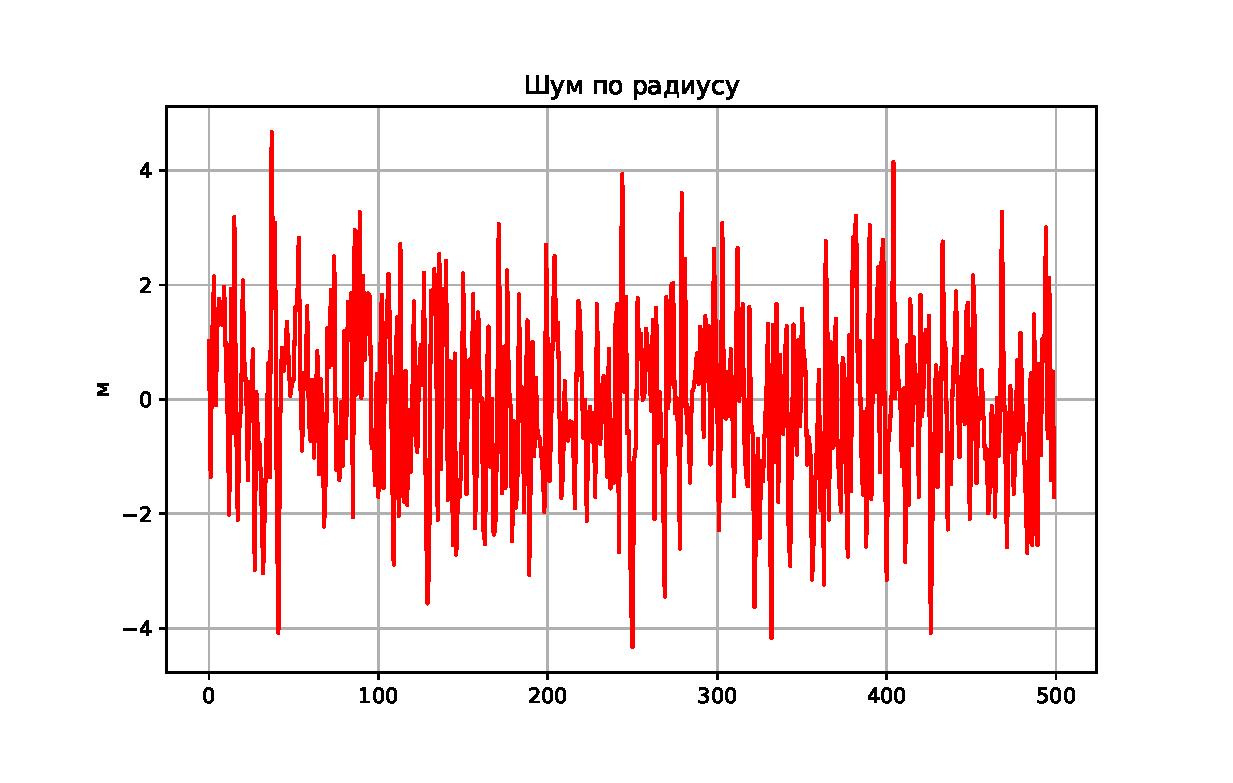
\includegraphics[width=1\linewidth]{images/kalmanfilter_noizeR.eps} \\ а)}
\end{minipage}
\hfill
\begin{minipage}[h!]{0.5\linewidth}
\center{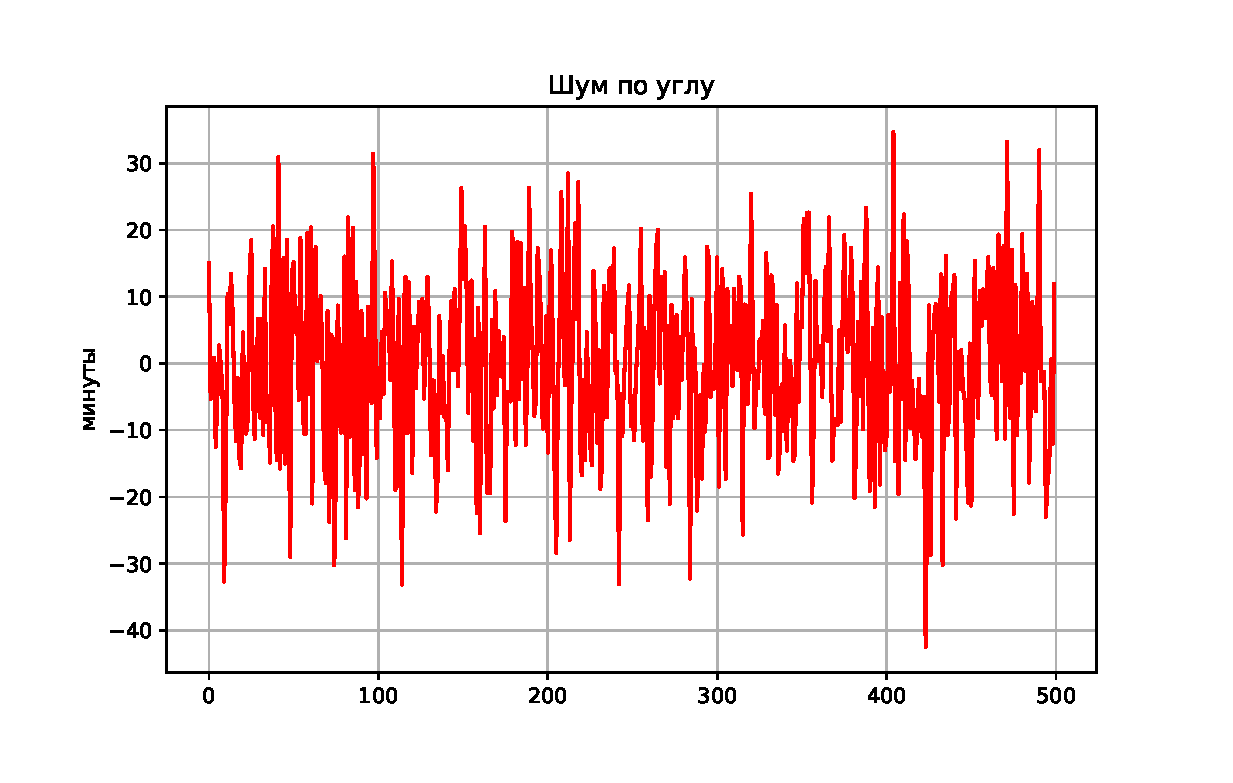
\includegraphics[width=1\linewidth]{images/kalmanfilter_noizeS.eps} \\ б)}
\end{minipage}
\caption {Графики шума от номера измерения а)  по радиусу ; б) по углу.}
\label{train}
\end{figure}


\begin{figure}[h!]
\begin{center}
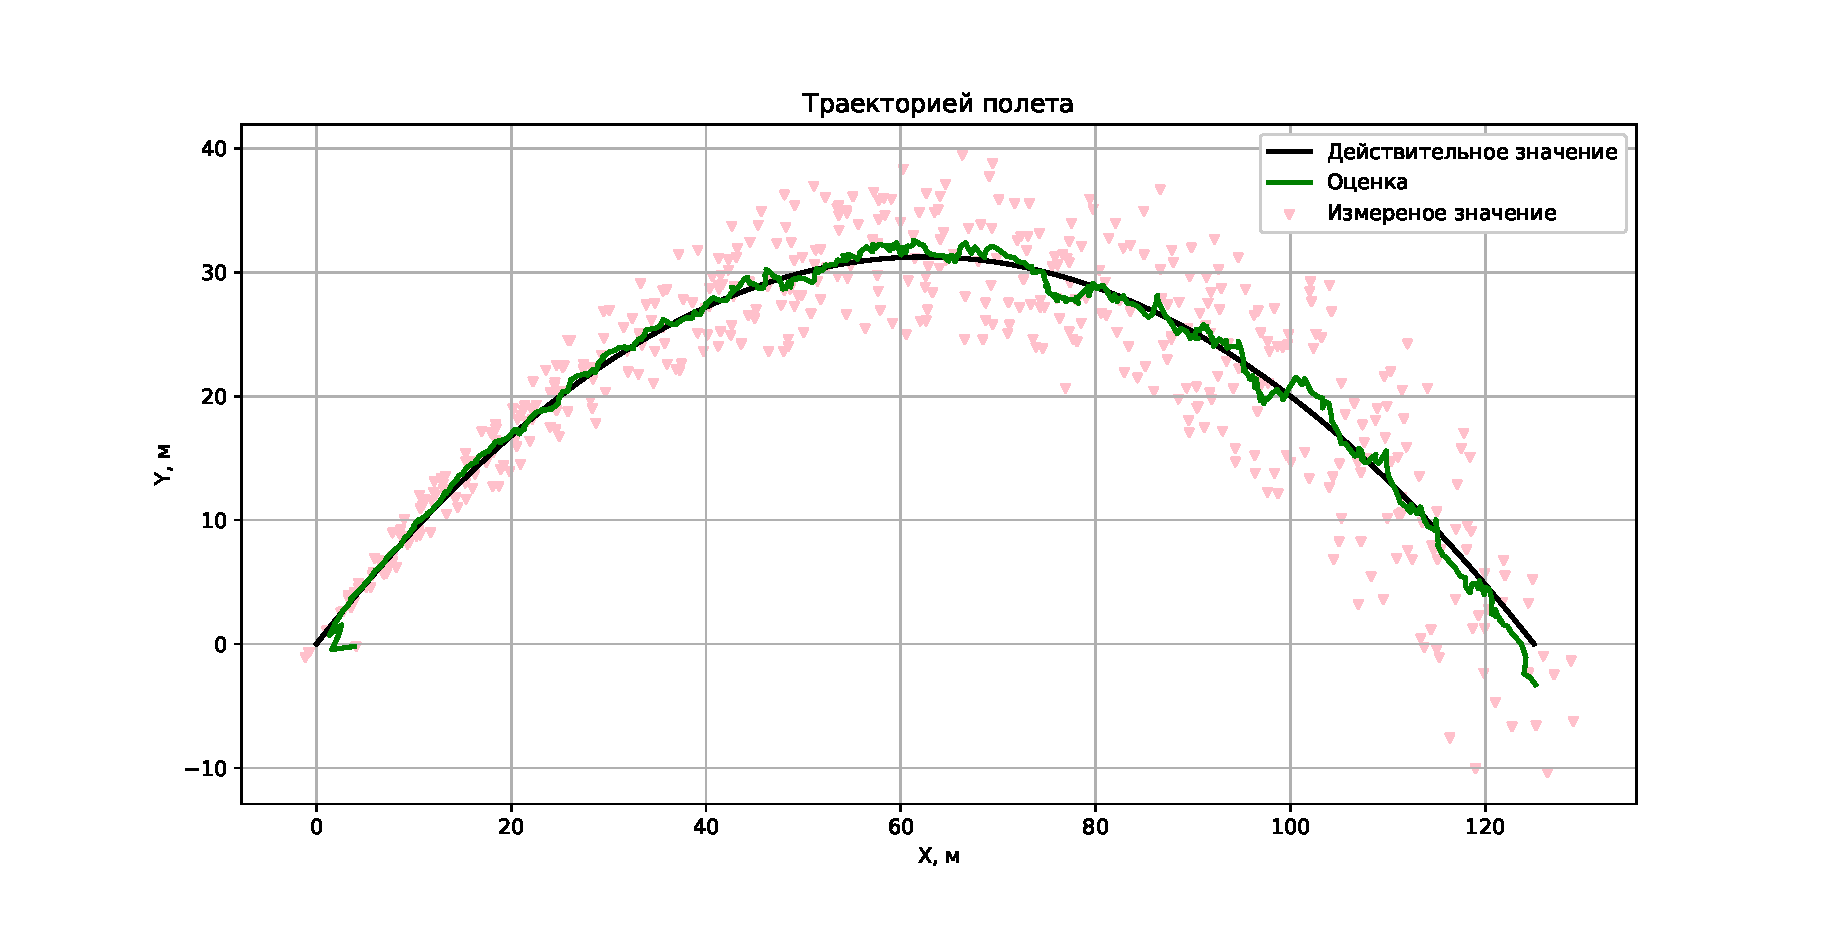
\includegraphics[width=0.8\textwidth]{images/kalmanfilter1.eps}
\end{center}
\caption{Полёт тела в плоскости $XY$} \label{kalman1}
\end{figure}

Качественно из рис. \ref{kalman1} видно, что фильтр очень качественно обрабатывает данные,  приближая их к истинным. Теперь выведем графики ошибок: \textit{измеренное значение - истинное значение} и \textit{оценочное значение - истинное значение}(рис.\ref{kalman2} и рис.\ref{kalman3}).

\begin{figure}[h!]
\begin{center}
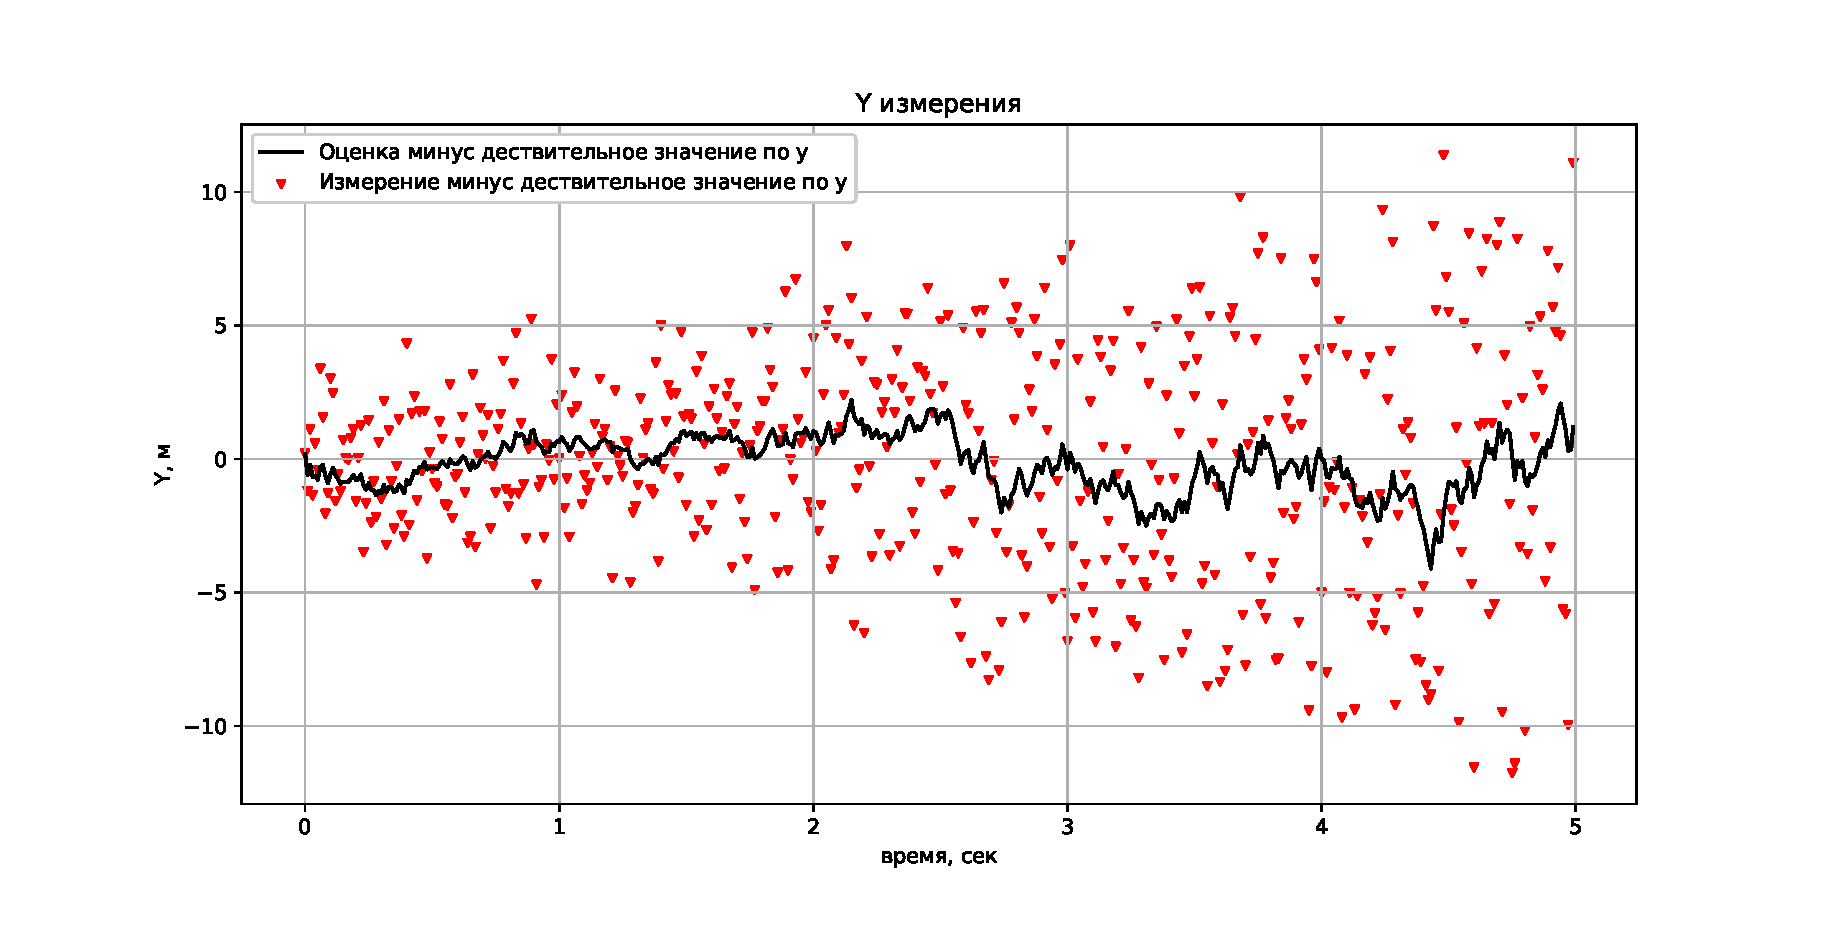
\includegraphics[width=0.8\textwidth]{images/kalmanfilter2.eps}
\end{center}
\caption{Отклонение по $Y$} \label{kalman2}
\end{figure}

\begin{figure}[h!]
\begin{center}
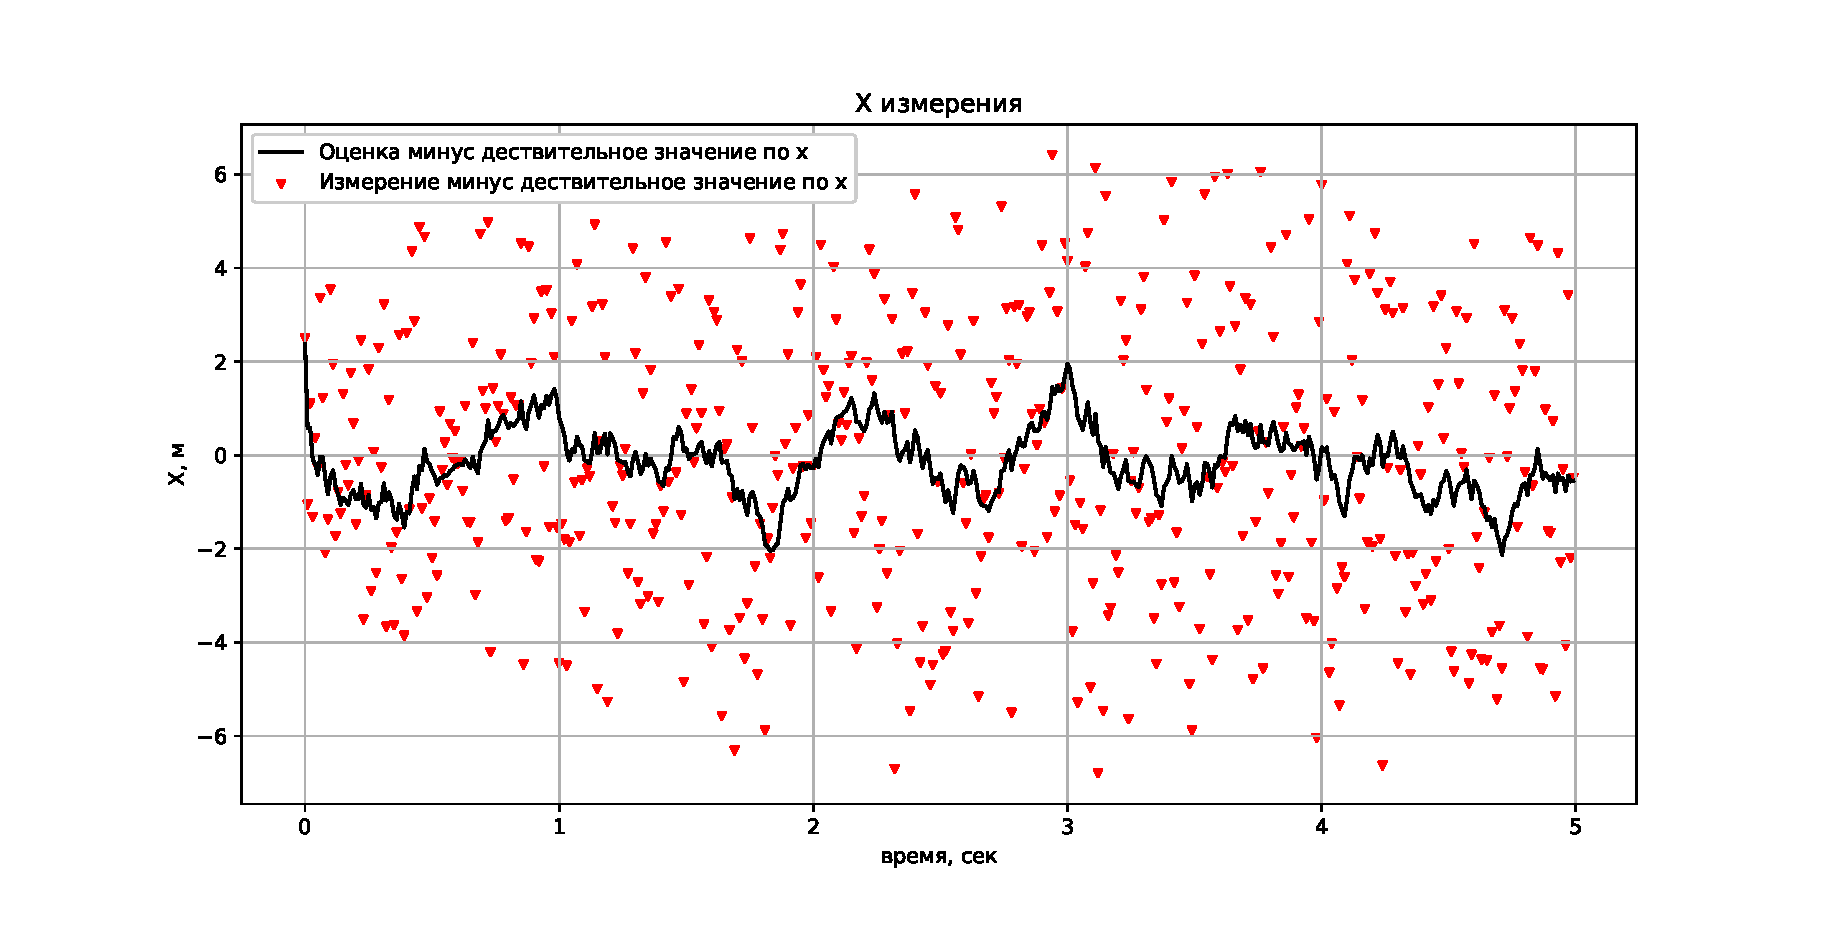
\includegraphics[width=0.8\textwidth]{images/kalmanfilter3.eps}
\end{center}
\caption{Отклонение по $X$} \label{kalman3}
\end{figure}
\newpage
Из графиков видно численно насколько точно воспроизводится фазовый вектор из полученных измерений.  Выведем также зависимости диагональных элементов в матрице ковариации $P$, соответствующих ошибкам по координатам $X$ (рис. \ref{kalman4}) и $Y$(рис. \ref{kalman5}):


\begin{figure}[h!]
\begin{center}
\includegraphics[width=0.8\textwidth]{images/kalmanfilter4.eps}
\end{center}
\caption{Среднеквадратичная ошибка по $X$} \label{kalman4}
\end{figure}

\begin{figure}[h!]
\begin{center}
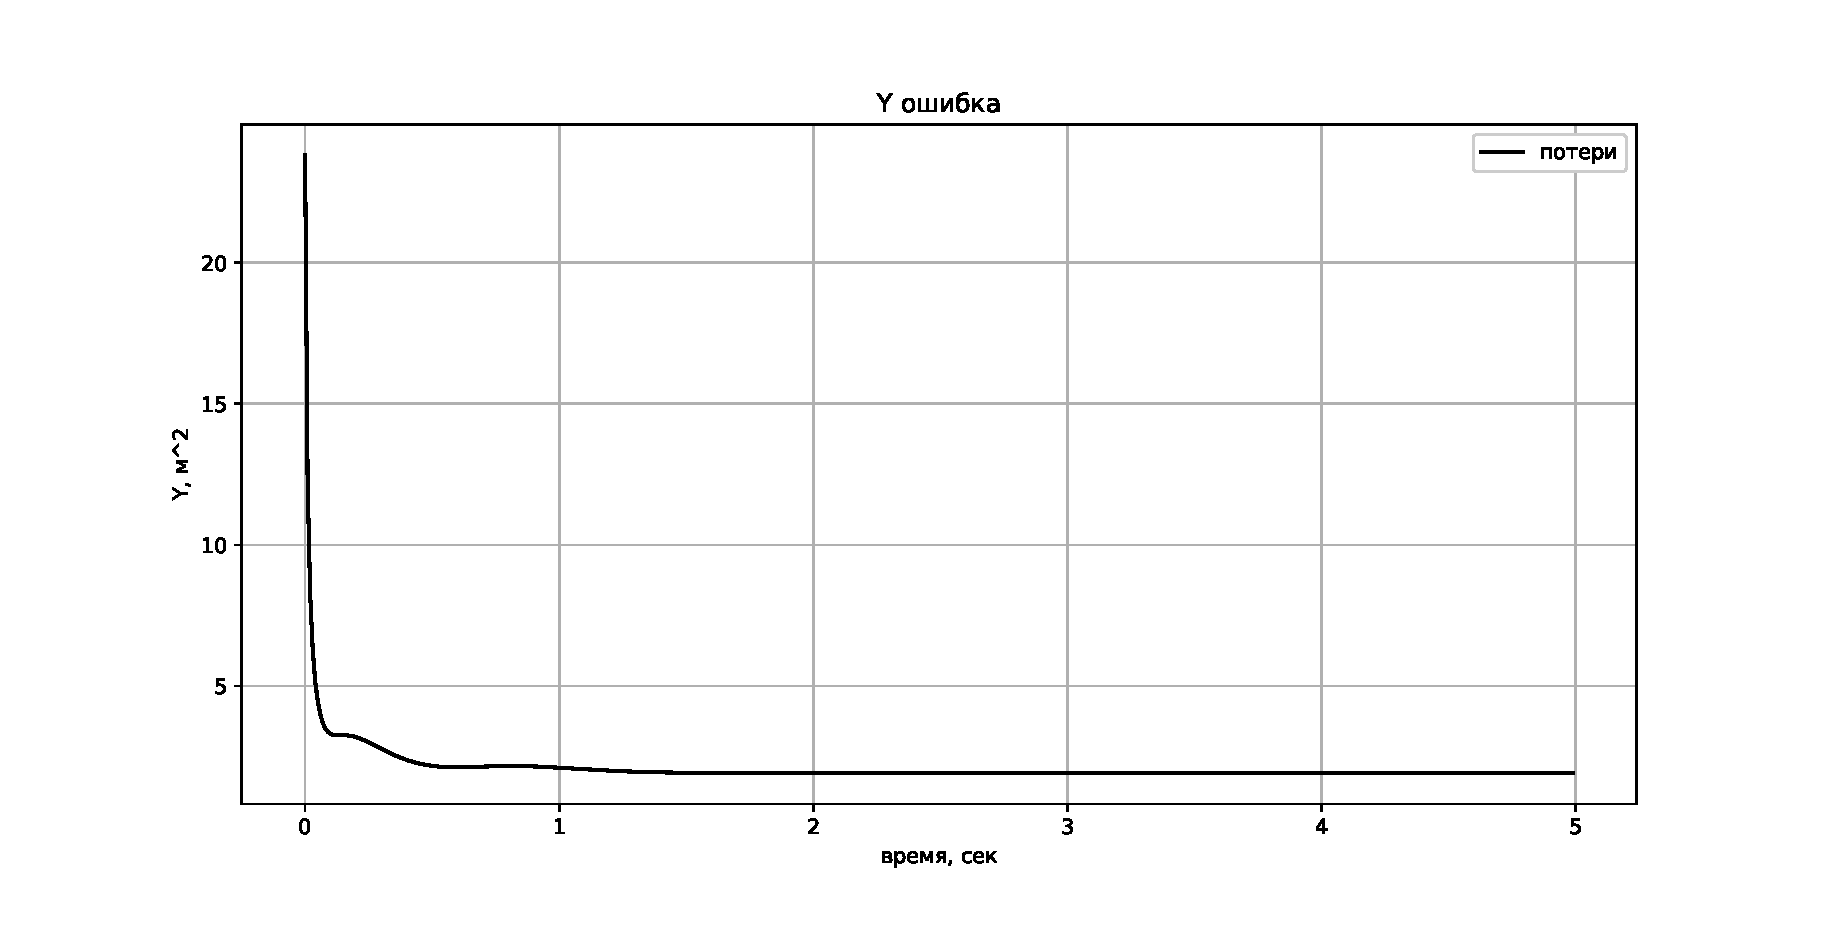
\includegraphics[width=0.8\textwidth]{images/kalmanfilter5.eps}
\end{center}
\caption{Среднеквадратичная ошибка по $Y$} \label{kalman5}
\end{figure}

\newpage
На графиках \ref{kalman4} и \ref{kalman5} видно, что ошибка определения траектории полёта падает,  т.е.  В процессе фильтрации алгоритм Калмана адаптируется к объекту обработки, что увеличивает точность экстраполяции значений и делает фильтр менее подверженному внешним шумовым факторам.

В следующих главах сравнение нового алгоритма фильтрации  будет вестись с построенной в данной главе моделью фильтра Калмана.  Будет изучаться реакция и основные характеристики обеих алгоритмов на траектории баллистических и гиперзвуковых объектов.

Теперь же обсудим основные выводы  по анализу и моделированию фильтра Калмана  рассматриваемого  до сих пор.
\newpage

\subsection{Результаты анализа и моделирования фильтра Калмана}
Сгруппируем важные свойства и выводы фильтра Калмана, которые необходимы для дальнейших рассуждений:
\begin{itemize}
\item Фильтр Калмана главным образом применяется для линеаризованных данных.  Следовательно, можно  считать его линейной моделью.
\item В алгоритме Калмана решается задача по минимизации среднеквадратичного отклонения между оцененным и истинным значениями;
\item Существует аналитическое решение из задачи по минимизации среднеквадратичного отклонения по поиску весовых коэффициентов в матрице $K$;
\item Высокое приближение фильтрованных данных к истинным.
\end{itemize}

Фильтр Калмана допускает линейность обрабатываемых данных, а также требует ручной настройки - задании внешних параметров обработки, что делает алгоритм ненадёжным при неизвестных характеристиках фильтруемых данных. А в совокупности с необходимостью на каждом шаге искать новую весовую матрицу $K$ путём вычисления обратной матрицы (формула \eqref{searchK}), алгоритм затрудняет поиск и  разработку аппаратно-программных решений по увеличению скорости фильтрации.  
По этим причинам возникает потребность, в новых алгоритмах обработки траекторий, которые могли бы самостоятельно адаптироваться к шумовым характеристикам данных, учитывая нелинейность самих траекторий, а также имели бы преимущество  по оптимизации в вычислительной сложности.

Одним из новых подходов в решении задачи определения траекторий полётов,  который рассматривается в работе, является применение нейронных сетей. Приступим к обсуждению основных принципов и преимуществ использования нейронных сетей.

\newpage
\section{Рекуррентные нейронные сети}
\subsection{Нейронная сеть}
Человеку и многим живым существам в каждый момент приходится решать задачи по  распознаванию, классификации и принятию решения, а также, используя результаты последствий принятых действий, обучаться.  Нейросетевой подход возник в результате попыток моделирования биологического алгоритма принятий решения -- мозга.

Впервые понятие нейронных сетей были введены и разработаны в алгоритмах  У. Маккалока и У. Питтса в 1943г.  \textbf{Нейронная сеть (NN --  англ.  neural network) или искусственная нейронная сеть, ИНС} -- математическая модель, построенная по принципу организации и функционирования биологических нейронных сетей -- сетей нервных клеток живого организма, которая последовательными линейными и нелинейными преобразованиями переводит объект из исходного признакового пространства в промежуточные или целевые(межслойные),а в конце и в итоговое пространство. 

Нейронные сети способны в отличие от других математических моделей(линейных моделей, логистических регрессий) распознавать сложные и нелинейные зависимости в структурированных данных (траектории движения также являются последовательными и структурированными данными). Все потому, что основной задачей нейронных сетей является сначала преобразование данных в новое информативное пространство,  а затем поиск решения на новом пространстве для поставленных условий.  Возможностью нейросетевого подхода стало появление и накопление достаточно большого количества данных, на которых возможно обучение нейронных сетей. 

Важными элементами в нейронных сетях являются линейная модель, нелинейные преобразования(функции активации) и метод обратного распространения ошибки, речь о которых будет в следующих главах.

Перед обсуждением структуры рекуррентных нейронных сетей,  далее именуемых RNN\footnote{RNN (англ.  recurrent neural network) -  рекуррентная нейронная сеть.}, рассмотрим более простые архитектуры и другие важные понятия,  необходимые в RNN

Основой любой NN\footnote{NN (англ.  neural network) -  нейронная  сеть.} является линейная модель.

\subsection{Линейные модели}

Линейная модель - это базисная конструкция,  которая по набору признаков  принимает решение об принадлежности или свойствах объекта,  которому они принадлежат.

$$Y=X_1+X_2+X_3,$$
$Y$ -  решение  системы,  $X_i$ - категориальные признаки\footnote{Многие методы предполагают, что все признаки $X\in R$. Однако, в некоторых задачах признаки могут принимать значения из множеств, не совпадающих с множествами вещественных чисел. Такие признаки называются категориальными, факторными или номинальными \cite{nnkategor}.}.

 Линейная модель решает задачи:
\begin{itemize}
\item Классификации - формализованная задача, в которой имеется множество объектов (ситуаций), разделённых некоторым образом на классы. Задано конечное множество объектов, для которых известно к каким классам они относятся. Это множество называется выборкой. Классовая принадлежность остальных объектов неизвестна. Требуется построить алгоритм, способный классифицировать произвольный объект из исходного множества (работа с дискретными величинами).
\item Регрессии - формализованная задача, в которой есть множество объектов, есть функция на нем. Для некоторого подмножества объектов задано значение функции. Нужно научиться предсказывать значение функции на других объектах. Качество выполнения задачи определяется функционалом качества. Например, MSE (работа с непрерывными величинами).
\end{itemize}

Подробнее о постановках задач классификации, регрессии и других задач в курсе лекций К. В. Воронцова\cite{voron}.  Мы же рассмотрим задачу линейной регрессии: 

$$\mathds{E}(Y|X)=f(X);$$

или

$$Y=f(X)=\varepsilon;$$

$f$ - функция регрессии, и для линейной модели имеет вид:

$$f_\omega(x)=\omega_0+\sum\limits_{i=1}^p\omega_ix_i\equiv x^T\omega;$$

где $\omega=(\omega_0,\omega_1,...,\omega_n)^T$ - веса, $x=(1,x_1,...,x_n)^T$- признаки объектов. 

Пусть теперь мы имеем  $n$ объектов: $(x^i,y^i)$ $i=\overline{1,n}$,  где $y^i\in R$ - метки  объекта,   $x^i\in R$ - описание  объекта.

Тогда матрицы  наших  объектов: $$X=[x^1,...,x^n]^T, X\in  R^{n\times p};\qquad Y=[y^1,...,y^n]^T, Y\in  R^{n}.$$

 \begin{equation}\label{Xw}
f_\omega(X)=X\omega=\widehat{Y};
\end{equation}
 
 Осталось только выбрать веса для  матрицы $\omega$. Введём функцию эмпирической ошибки,  как сумму всех наших потерь:
 
 $$\text{Empirical risk}=\sum\limits_\text{by objects}\text{Loss on object}.$$
 
И будем её минимизировать по весам $\omega$,  то есть:

$$Q(X)=\sum\limits_{i=1}^{n}L(y^i,f_\omega(x^i))\longrightarrow\min$$

 Таким образом мы сможем,  подбирать $\omega$. 
 
 В общей сложности для разных задач  существуют разные функции потерь. В данной работе (в задачи регрессии) будет использоваться функция среднеквадратичного  отклонения:
 \begin{equation}\label{MSE}
\text{MSE loss: } L(y_t,y_p)=(y_t-y_p)^2.
\end{equation}
 
Тогда:

$$Q_\text{MSE}=(Y-X\omega)^T(Y-X\omega)\longrightarrow\min;$$

Для минимизации исследуем функцию потерь,  взяв производную:

$$\nabla_\omega Q_\text{MSE}=-2Y^TX+2X^TX\omega^T=0.$$

Откуда матрица весов:
\begin{equation}\label{w}
\omega^*=(X^TX)^{-1}X^TY;
\end{equation}

По  Теорема Гаусса — Маркова\cite{voron},  данная матрица единственна.  В данной постановке задачи и в выводе её решения,  чётко прослеживается аналогия с линейной  моделью фильтра  Калмана,  откуда можно сделать вывод, что фильтр Калмана - это модель  задачи линейной  регрессии.

Как видно из формулы \ref{w}, решение $\omega^*$ не устойчиво, так как матрица  $X^TX$ не всегда имеет обратную.  Тут следует  дополнить  задачу и  потребовать  от неё устойчивости в решении - провести  регуляризацию.  Добавим к нашей функции  ошибки вторую  норму матрицы  весов, умноженную на квадрат коэффициента $\lambda$:

$$L_2=||Y-X\omega||^2_2+\lambda^2||\omega||^2_2$$ 
$$\omega^*=(X^TX+\lambda^2I)^{-1}X^TY;$$

 Данный метод регуляризации (сдвиг решения) называется $L_2$ регуляризацией или регуляризацией Тихонова\cite{Spokbook}.  Существует также $L_1$  регуляризация - регуляризация через манхэттенское расстояние\cite{lasso}.  
 
Описанное выше аналитическое решение включает в себя инверсию матрицы $X^T X$ (или $X^T X + \lambda I$), что довольно дорого с точки зрения вычислительных ресурсов. Сложность инверсии матрицы можно оценить как $O (p^3 + p^2 N)$. Это приводит нас к итеративным методам оптимизации, которые являются более эффективными и фактически являются основным подходом к оптимизации в машинном обучении.

Градиентный спуск - один из самых популярных методов оптимизации. Стоит отметить тот факт, что цель минимизации (максимизации) (например, значение функции потерь) должна быть дифференцируема по параметрам модели.  Используя градиентный спуск, вектор весов $\mathbf{w}^{(t+1)}$ на шаге $t+1$ можно выразить в следующем виде:

$$
\mathbf{w}^{(t+1)} = \mathbf{w}^{(t)} - \eta_t \nabla Q(\mathbf{w}^{(t)}),
$$
где $\eta_t$ шаг градиента (называемый \textit{learning rate}(англ.)).

Градиент в случае функции потерь MSE принимает следующий вид:

$$
\nabla Q(\mathbf{w}) = -2X^TY + 2X^TX\mathbf{w} = 2X^T(X\mathbf{w} - Y).
$$

В этом случае сложность составляет всего $O (pN)$. Чтобы сделать его еще более эффективным,  мы будем использовать стохастический градиентный спуск,  который вычисляет градиент только по некоторому случайному подмножеству данных(англ. batch) $K$ точек, так что конечная сложность уменьшается до $O(pK)$, где $K << N$.

Данный процесс,  когда градиентным спуском нашей функции ошибки подбирается матрица весов  $\omega$,  называется обучением (англ.training).

\subsection{Функции активации}
Линейные модели отлично себя проявляют в классификации или  в регрессии  \textbf{линейных} данных,  показывают также достойные  результаты  с данными,  которые неплохо аппроксимируются прямой.  Например, малый участок зашумленной траектории,  обрабатываемый фильтром Калмана. 

Однако, большенство данных (траектория движения), плохо или вообще не аппроксимируются прямой, так как имеют другие  зависимости(например логарифмические),  поэтому нам необходимо <<уйти>>  от \textit{нелинейного} признакового пространства в новое пространство(чаще всего  линейное), где мы сможем работать  с  новыми  признаками  знакомыми способами.  Идея  очень проста,  добавим \textbf{нелинейное преобразование}:

\begin{enumerate}
\item Входные данные: $X$;
\item Линейная модель: $h=X\omega$;
\item Нелинейное преобразование: $\sigma(h)$;
\item MSE;
\item Предсказание.
\end{enumerate}

Нелинейную функцию, в частности $\sigma$,  называют \textbf{функцией  активации}. Функций активаций бывает множество  видов,  приведем в  качестве примера пару из них:

\begin{itemize}

\item $\sigma(x)=\frac{1}{1+e^{-x}},$ $R\longrightarrow(0,1)$;

\item $\th(x)$,  $R\longrightarrow(-1,1)$;

\item $\ln(1+e^x)$,  $R\longrightarrow(0,\infty)$;

\end{itemize}

Функции активации  позволяют  нашей сети,  переводить признаки  в новое  удобное для себя  пространство,  где NN сможет с ними работать или перевести в еще одно признаковое пространство.  Множество таких линейных и  нелинейных преобразований называются  слоями.  Присуствие функций активации в преобразованиях NN является одной из отличительных черт,  почему NN превосходит классические линейных модели в работ с нелинейными данными.

Для работы NN обычно имеет в каждом слое(преобразование) обучаемый параметр или несколько, а также требует, чтобы все слои имели производную в точке, для возможности  обучаться градиентным  спуском.

\textbf{Примечание.}

Название и происхождение функций активации уходит в биологию и психологию.  Когда люди решили смоделировать поведение  \textit{нейронов},  они обнаружили, что множество  нейронов передают  потенциал одному,  и тот, после превышения порогового значения(\textit{активации}),  начинает передавать накопившийся потенциал остальным.  То есть для работы модели нейронов  или нейронной сети требуется функция  активации,  которая была бы  <<дифференцируема>>.  Первой такой функцией стала  $\sigma$.

\subsection{Метод обратного распространения ошибки}
Скажем пару слов об методе обратного распространения ошибки.  Данный метод является методом вычисления градиента, для обновления весов в  многослойной нейронной сети. Главным принципом явлется вычисление производной в точке сложной функции. 

Рассмотрим нейронную сеть из пары слоев:
\begin{enumerate}
\item Входные данные: $X$;
\item Линейная модель: $h=X\omega$;
\item Нелинейное преобразование: $\sigma(h)$;
\item MSE;
\item Предсказание.
\end{enumerate}
На этапе поиска ошибки(MSE формула \eqref{MSE}) идет обучение нейронной сети, ставится задача минимизации потерь:
$$MSE=L\longrightarrow\min.$$
Для этого необходимо посчитать производную от $L$ по параметрам обучения--весам, и  приравнять к нулю.
$$\frac{\partial L}{\partial \omega}=0.$$ 
Но $L$ сложная функция от $\omega$, так как $L(\sigma(\omega))$, тогда производная будет считаться по формуле:
$$\frac{\partial L}{\partial \omega}=\frac{\partial L}{\partial\sigma}\frac{\partial\sigma}{\partial\omega}.$$ 
Зная численное значение вложенных функций в точке, производная сложной функции ищется  произведением найденного значения последних производных($\partial L/\partial\sigma$) на расчитанное значение следующей производной($\partial\sigma/\partial\omega$).  После  нахождение необходимой производной производим обновление весовых параметров:

$$\omega_{n+1}=\omega_n-\eta \frac{\partial L}{\partial \omega}$$


\subsection{Рекуррентная нейронная сеть (RNN)}
Чаще всего данные,  которые встречаются, и которые необходимо обрабатывать,  обладают структурностью.  Например, речь,  где порядок слов и букв обладает собственной архитектурой и несёт важную информационную нагрузку.  При обработке тут важно учитывать свойства структурности информации.  

Траектория движения имеет последовательность точек,  которые привязаны ко времени,  это означает,  что каждая последующая координата зависит от совокупности предыдущих.  То есть при фильтрации новых значений помимо знаний о физической природе объекта можем пользоваться доступным контекстом - уже обработанными точками траектории. 

\subsubsection{Схема RNN}

\begin{figure}[h!]
\begin{center}
\includegraphics[width=0.9\textwidth]{images/RNN1}
\end{center}
\caption{Схема RNN loop\cite{NN}.} \label{RNN1}
\end{figure}

Пусть уже имеются данные и часть контекста,  связанного с ними. Теперь <<обогатим>> контекст следующими данными,  и получим результат обработанных значений в совокупности с предыдущими.  Для этого можно представить свои данные в виде векторов:  $C$ - контекст фиксированной размерности,  $i$  -  входные данные фиксированной размерности.  Для объединения старой и полученной информации можно конкатенировать вектора  $C$ и $i$ в $[C,i]$.  Для получения новых данных(нужной размерности) можно провести линейное преобразование: $W\cdot[C,i]+b$.  Нейронной сети необходимо иметь нелинейность в своих преобразованиях, поэтому добавим функцию активации после линейного слоя: $\sigma(W\cdot[C,i]+b)$.  Получили композицию преобразований, способную называться нейронной сетью, так как в ней имеется нелинейность в преобразованиях, и веса $W$ для обучения.  Скажем, что  $W\cdot[C,i]+b$ порождает вектор размерности, соответствующей изначальному контексту $C$,   следовательно, получаем обновленный контекст,  способный участвовать в дальнейшей циклической обработке данных.  Нейронные сети данного типа,  называют реку рентными,  а один оборот процесса - петлёй (англ.  loop), рис.  \ref{RNN1}.

\begin{figure}[h!]
\begin{center}
\includegraphics[width=1\textwidth]{images/RNN2}
\end{center}
\caption{Простейшая схема RNN\cite{NN}.} \label{RNN2}
\end{figure}

На  рис. \ref{RNN2} показана схема циклической работы RNN.

Можно заметить, что первоначальная информация вектора контекста после нескольких циклов добавления новых данных быстро <<забывается>> из-за фиксированной размерности $C$, и мы теряем картину начальных событий.  Учитывая, что в данных может присутствовать много зашумленных или ненужных значений,  имеет смысл запоминать важную информацию и пропускать остальную - дать нашей сети  возможность выбирать что нужно запомнить, а что  нет.

\subsubsection{Рекуррентная нейронная сеть с кратковременной,  долговременной памятью и уравнением экстраполяции Калмана} \label{KalmanLSTM}

LSTM (англ.  Long Short-Term Memory) - рекуррентная нейронная сеть с кратковременной и долговременной памятью\footnote{Основной материал по LSTM можно найти в лекции Стэнфорда \cite{RNN}}.  Основная структура схемы LSTM на  рис.  \ref{RNN3}.

\begin{figure}[h!]
\begin{center}
\includegraphics[width=1\textwidth]{images/RNN3}
\end{center}
\caption{LSTM\cite{RNN}.} \label{RNN3}
\end{figure}
В схеме используется функция активации $\tanh$,  позволяющая держать распределение данных в интервале $(-1,1)$,  а также центрировать их относительно $0$,  поэтому $\tanh$ не перегрузится от больших значений, а градиент не взорвется.\footnote{Взрыв градиента - понятие, когда градиент быстро растёт и вызывать переполнение данных.} 

\begin{figure}[h!]
\begin{center}
\includegraphics[width=1\textwidth]{images/RNN4}
\end{center}
\caption{LSTM loop\cite{RNN}.} \label{RNN4}
\end{figure}

LSTM использует два вектора контекста: $С$  - долговременная память, $h$ - кратковременная память.  Задача выбора: какую информацию оставить, а какую забыть,  является бинарной классификацией. $f_t$ - вектор "забывания" содержит $0$ в своих местах,  где  данные нужно стереть,  и  $1$,   где сохранить:

$$f_t=\sigma(W_f\cdot[h_{t-1},x_t]+b_f).$$

Функция  $\sigma$ бинарно классифицирует данные $(0,1)$ , после чего совершается поэлементное умножение $f_t$ на  $C_{t-1}$. Теперь нужно запомнить новую информацию для этого, снова решаем задачу классификации, пусть $i_t$ - вектор "запоминания" аналогичный $f_t$:

$$i_t=\sigma(W_i\cdot[h_{t-1},x_t]+b_i).$$

А также нужны сами данные $\widetilde{C}_t$ для запоминания:

$$\widetilde{C}_t = \tanh(W_C\cdot[h_{t-1},x_t]+b_C).$$

Обновление долговременной памяти:

$$C_t=f_t\cdot C_{t-1}+i_t\cdot \widetilde{C}_t.$$

Изменение краткосрочной памяти,  аналогично $C_t$:

$$o_t=\sigma(W_o\cdot[h_{t-1},x_t]+b_o);$$

$$h_t=o_t\cdot\tanh(C_t).$$
 
 Для решения задачи фильтрации в алгоритме Калмана заменим пункт \textbf{Обновления}  формулы \ref{K}, \ref{KP} на LSTM.  Сеть  будет получать зашумленный сигнал $x_{\text{noise}_t}$, выводить уже отфильтрованное значение $h_t$. Далее по формулам \ref{xFuB} на основе предыдущего значения фильтрации,  пользуясь свойствами физической модели объекта, предсказываем предположительное значение $\widetilde{x}_t$.  Конкатенируем $[\widetilde{x}_t,h_t]$ и совершаем линейное преобразование,  получая вектор  размерности  координат точки:
 
$$\widetilde{x}_t =Fx_{t-1};$$

\begin{equation}\label{KRNN}
x_t=W_K\cdot[\widetilde{x}_t,h_t]+b_k.
\end{equation}


\begin{figure}[h!]
\begin{center}
\includegraphics[width=1\textwidth]{images/RNN5}
\end{center}
\caption{Обучение во времени.} \label{RNN5}
\end{figure}

Последний линейный слой (формула \ref{KRNN}),  описанный выше, также будет обучаться нейронной сетью, так как является её частью. Подбирать весовые параметры NN будем методом стохастического градиентного спуска от Loss функции \ref{MSE}(фильтрация сигнала - задача регрессии),считая производные слоев\cite{mtrixgrad} рис.  \ref{RNN5}.

Практическую реализацию модели на Python можно смотреть в \hyperref[appendix]{Приложении}.
\newpage
\section{Реализация}

Рассмотрим основной алгоритм фильтра.

Архитектура сети уже обсуждалась в разделе \hyperref[RNNfilter]{Фильтр Калмана и LSTM}. Рассмотрим в общем плане практическую реализацию.  Нейронная сеть написанна на основе фреймворка машинного обучения PyTorch с открытым исходным кодом.  

Создаем класс данных(основанный на стандартах Dataset PyTorch), предварительно  приводя его в стандартизированный вид фиксированной длинны.

\begin{lstlisting}
class ModuleRNN(nn.Module)
\end{lstlisting}
Класс нейронной сети, который содержит в себе главную архитектуру системы. В методе forward описан алгоритм, обсужденный в главе \hyperref[RNNfilter]{Фильтр Калмана и LSTM}:

\begin{lstlisting}[label=some-code,caption=ModuleRNN.forward(), language=Python]
def forward(self, new_data, flash_memory, short_term_memory, long_term_memory, F):

        memory = torch.cat([new_data, short_term_memory], dim=-1)

        forgetfulness = torch.sigmoid(self.rnn_forget(memory)) #forgetting dataforgetting data
        conservation = torch.tanh(self.rnn_save(memory)) #the acquisition of new data
        information = torch.sigmoid(self.rnn_data_selection(memory))

        long_term_memory = (forgetfulness * long_term_memory) + (information * conservation)

        short_term_memory = torch.sigmoid(self.rnn_quick_overview(memory)) * torch.tanh(long_term_memory)
        
        with torch.no_grad():
            flash_memory = self.predict_Kalman(F, flash_memory)
            flash_memory_grad = flash_memory[:,0::3]


        predicted_data = self.rnn_prediction(torch.cat([flash_memory_grad, short_term_memory], dim=-1))

        with torch.no_grad(): 
            flash_memory[:,0::3] = predicted_data

        return predicted_data, flash_memory, short_term_memory, long_term_memory
\end{lstlisting}

В коде имеются области with torch.no\_grad(), отключающие поиск производных для вошедших в них операций, так как они не являются дифференцируемыми\footnote{Cрезы тензоров используются для оптимизации, так как являются более быстрыми и эффективными операциями чем  матричные умножения}.

\begin{lstlisting}
def rnn_loop()
\end{lstlisting}

Главный цикл в котором работает RNN.

 \subsection{Фильтрация траекторий баллистических измерений}

\subsubsection{Обучение и проверка точности}\label{trainval}

Приведём процесс обучения и проверка точности(валидации\footnote{Валидация - это проверка данных на соответствие заданным условиям и ограничениям.}) в виде графиков  зависимостей  от эпох\footnote{Эпоха - время, за которое обрабатываются все данные.}:
\begin{figure}[h]
\begin{minipage}[h]{0.49\linewidth}
\center{\includegraphics[width=1\linewidth]{images/losstrain.eps} \\ а)}
\end{minipage}
\hfill
\begin{minipage}[h]{0.49\linewidth}
\center{\includegraphics[width=1\linewidth]{images/valtrain.eps} \\ б)}
\end{minipage}
\caption{Процесс обучения и валидации. а) график зависимости средней по данным MSE ошибки от эпохи; б) график зависимости средней по данным точности от эпохи.}
\label{train}
\end{figure}

Напомним, что подбираем веса параметров NN методом стохастического градиентного спуска от функции потерь MSE \footnote{MSE - функция потерь (англ. loss), среднеквадратичная ошибка.}(формула \ref{MSE}):
$$\text{MSE loss: } L(y_t,y_p)=(y_t-y_p)^2.$$
Подсчет потерь ведется по формуле:
\begin{equation}\label{loss}
loss = \sqrt{\frac1S{\sum{(\mathbf{\widehat{x}}-\mathbf{x_\text{real}})^2}}},
\end{equation}
где $\mathbf{\widehat{x}}$ -- вектор оценочных значений  фазового вектора, $\mathbf{x_\text{real}}$-- действительный фазовый вектор,  $S$ --   колличество элементов в фазовом векторе.  Сначала находится поэлементная разница  двух векторов,  потом поэлементное возведение в квадрат.  Элементы полученного вектора скалываются и делятся на их общее количество. Далее идет  извлечение корня.

"Точность" осуществляем подсчетом количества точек фильтрованного сигнала, отклонившихся  от оригинала не  более чем на $5\%$. То есть сначала вычитается поэлементно из оцененного вектора действительный фазовый вектор. Полученная разница поэлементно делится на действительный вектор, а затем поэлементно логически сравнивается с критерием($D$). Получается вектор из  единиц и нулей, после суммирования всех элементов вектора, имеем общее число  координат,  удовлетворивших критерию. Данное число делится на общее число всех элементов. Итоговое значение - это среднее число оцененных координат удовлетворивших критерию.

\begin{equation}\label{accuracy}
accuracy =  \frac1S{\sum{\left(\frac{| \mathbf{\widehat{x}}-\mathbf{x_\text{real}}|}{\mathbf{x_\text{real}}}\leqslant D\right)}},
\end{equation}
где $\mathbf{\widehat{x}}$ -- вектор оценочных значений  фазового вектора, $\mathbf{x_\text{real}}$-- действительный фазовый вектор,  $D = 0,05$ -- допустимая ошибка $5\%$, $S$ --   колличество элементов в фазовом векторе.



\textbf{Вывод:} Из падения графиков на MSE и росте на Accuracy видно,  что сеть обучается. Точность на валидации чуть выше $81\%$, это связано с регуляризацией\footnote{В данном случае говорится об  секуляризации Dropout.} модели.

\newpage
\subsubsection{Проверка модели на контрольных данных}
Приведём проверку обученной модели на контрольных данных(тестирование) в виде графиков:
 \begin{figure}[h]
\begin{minipage}[h]{0.49\linewidth}
\center{\includegraphics[width=1\linewidth]{images/losstest.eps} \\ а)}
\end{minipage}
\hfill
\begin{minipage}[h]{0.49\linewidth}
\center{\includegraphics[width=1\linewidth]{images/valtest.eps} \\ б)}
\end{minipage}
\caption{Процесс тестирования. а) график зависимости средней по данным MSE ошибки от эпохи; б) график зависимости средней по данным точности от эпохи.}
\label{test}
\end{figure}

Потери и точность считаем  по формулам из предыдущей главы \eqref{loss}, \eqref{accuracy}(гл. \hyperref[trainval]{"Обучение и проверка точности"})
Ошибка в среднем $1,18$ км по траекториям.  А точности $5\%$ в среднем достигается в $79,0\%$  фильтрации.

\textbf{Вывод:} Сеть обучилась на наших данных, но возможен рост характеристик точности при  увеличении  обучающей выборки и количества весовых параметров.
 
\newpage
\subsubsection{Сравнение результатов фильтраций}
На данный момент уже разобраны фильтр Калмана и фильтр, с применением рекуррентной нейронной сети.  Сравним результаты фильтраций траекторий полетов баллистических снарядов, уже привычными,  функциями \eqref{loss}, \eqref{accuracy} (из главы \hyperref[trainval]{"Обучение и проверка точности"}):
$$
loss = \sqrt{\frac1S{\sum{(\mathbf{\widehat{x}}-\mathbf{x_\text{real}})^2}}},
$$
$$
accuracy =  \frac1S{\sum{\left(\frac{| \mathbf{\widehat{x}}-\mathbf{x_\text{real}}|}{\mathbf{x_\text{real}}}\leqslant D\right)}},
$$
где $\mathbf{\widehat{x}}$ -- вектор оценочных значений  фазового вектора, $\mathbf{x_\text{real}}$-- действительный фазовый вектор,  $D = 0,05$ -- допустимая ошибка $5\%$, $S$ --   колличество элементов в фазовом векторе.

\begin{figure}[h!]
\begin{center}
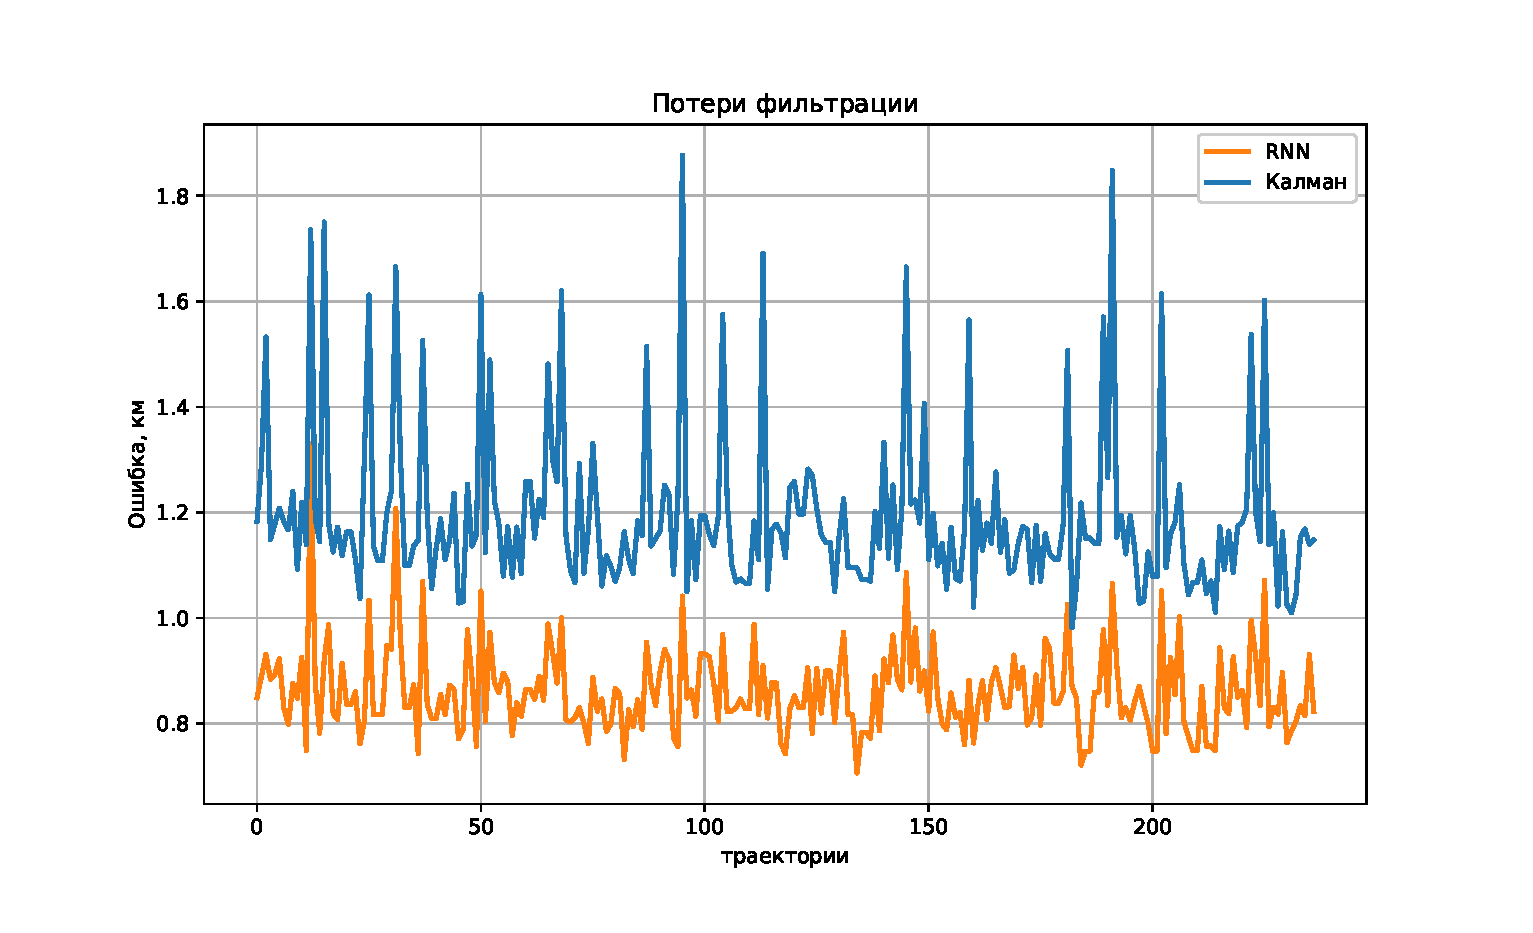
\includegraphics[width=0.6\textwidth]{images/battle1.eps}
\end{center}
\caption{Средние MSE потери по траекториям} \label{battle1}
\end{figure}

Средние по траекториям потери RNN фильтра Калмана составляют $0,9$ км,  тогда как у классического девяти-мерного фильтра они равны $1,2$ км.

\begin{figure}[h!]
\begin{center}
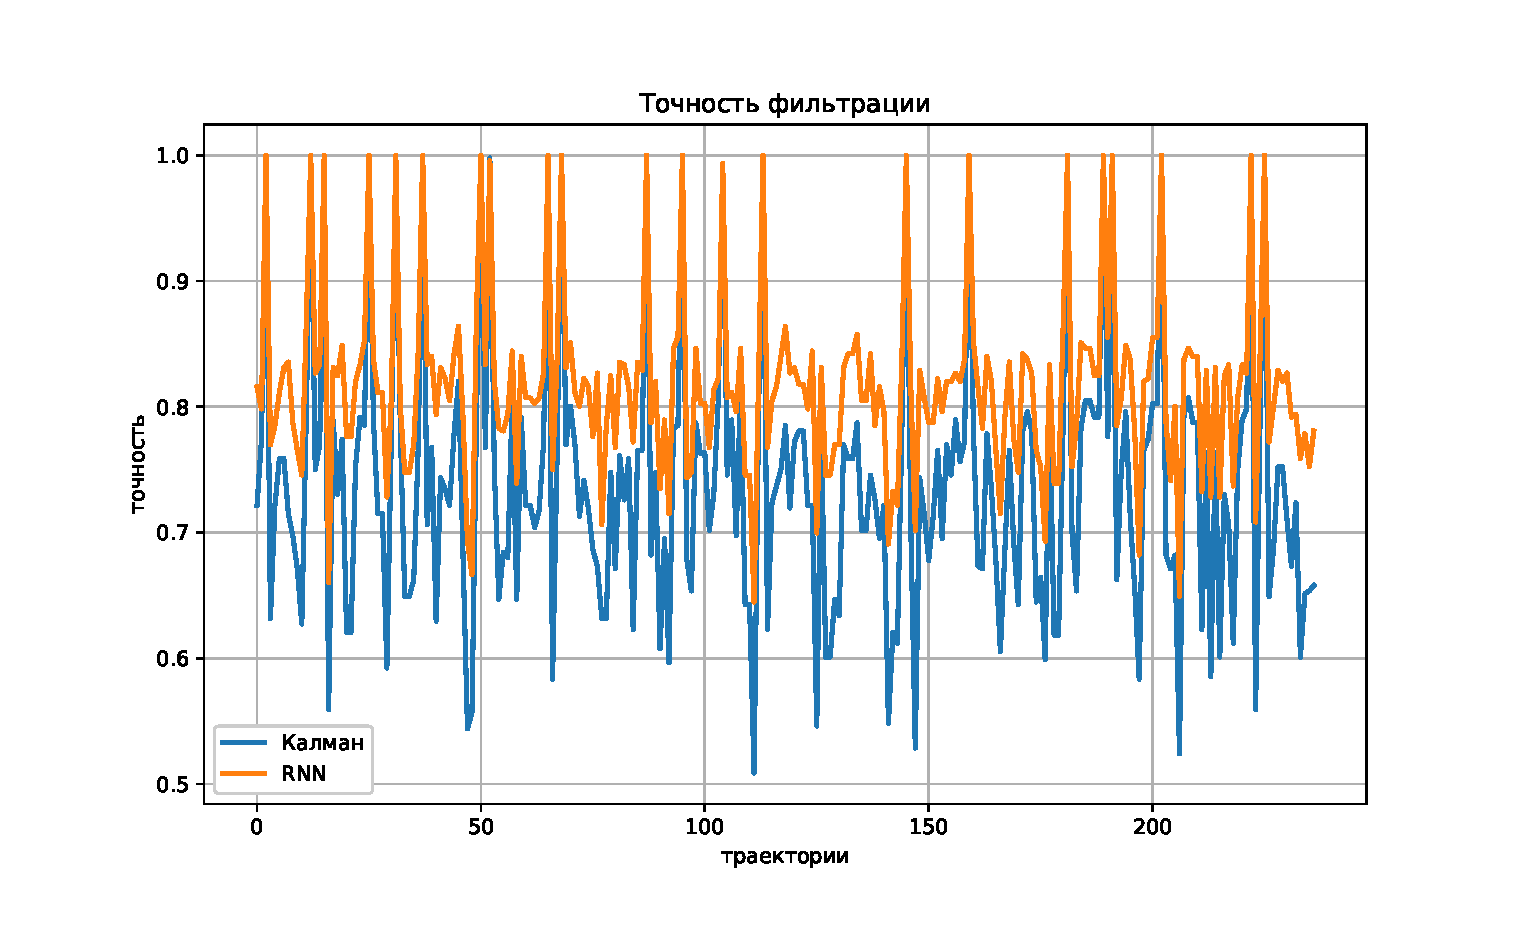
\includegraphics[width=0.6\textwidth]{images/battle2.eps}
\end{center}
\caption{Средняя точность по траекториям} \label{battle2}
\end{figure}

В $5\%$-ую точность в среднем по траектории попадают $81\%$ результатов фильтрации RNN,  и $73\%$ для фильтра Калмана. 

Для исследования характеристик  фильтров, также рассмотрим их работу не в среднем, а на конкретной произвольной траектории.  Будем выводить графики вида: |<<сигнал>>-<<сигнал+шум>>| и рядом |<<фильтрованный сигнал>>-<<сигнал+шум>>| в зависимости от времени.

 \begin{figure}[h]
\begin{minipage}[h]{0.49\linewidth}
\center{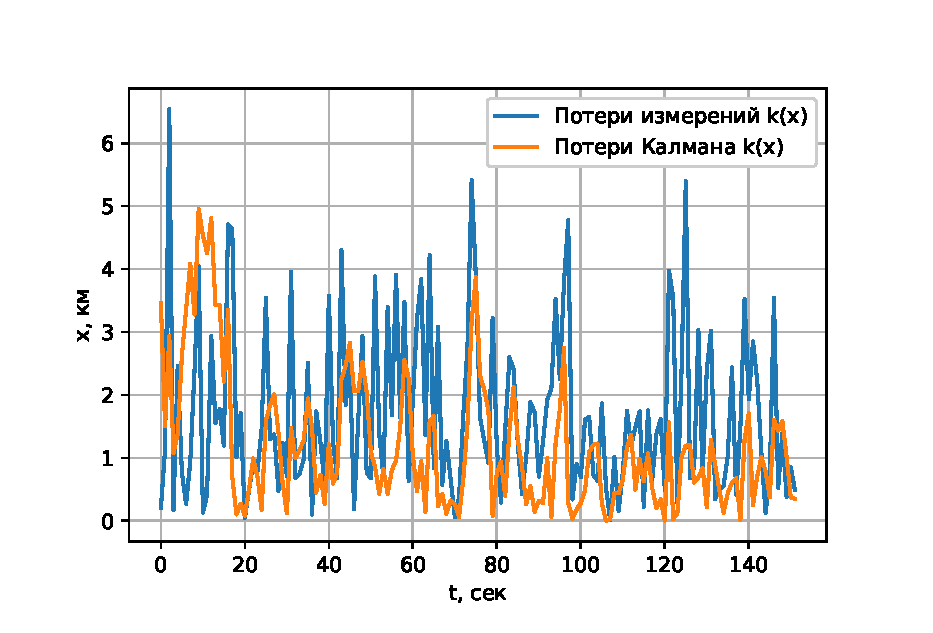
\includegraphics[width=1\linewidth]{images/kalmanx.eps} \\ а)}
\end{minipage}
\hfill
\begin{minipage}[h]{0.49\linewidth}
\center{\includegraphics[width=1\linewidth]{images/nnx.eps} \\ б)}
\end{minipage}
\caption{Графики ошибки по оси $x$. а) для классического фильтра Калмана; б) для фильтра Калмана с NN.}
\label{batlx}
\end{figure}

 \begin{figure}[h]
\begin{minipage}[h]{0.49\linewidth}
\center{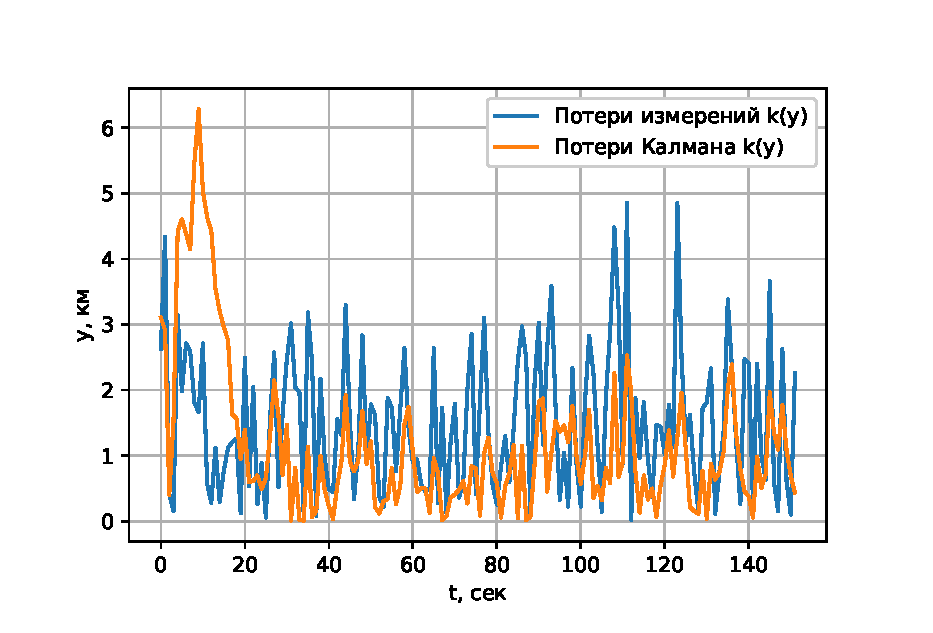
\includegraphics[width=1\linewidth]{images/kalmany.eps} \\ а)}
\end{minipage}
\hfill
\begin{minipage}[h]{0.49\linewidth}
\center{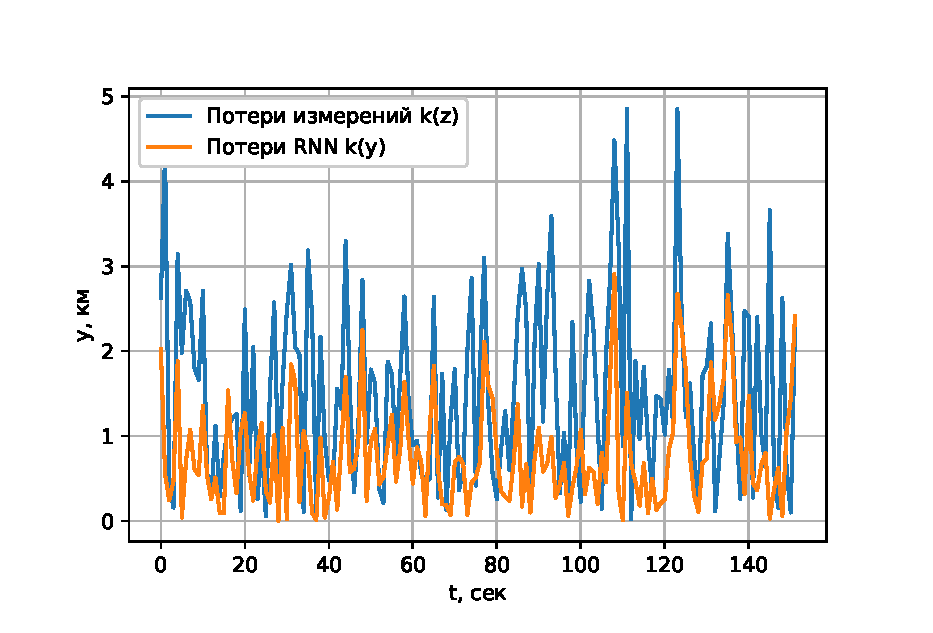
\includegraphics[width=1\linewidth]{images/nny.eps} \\ б)}
\end{minipage}
\caption{Графики ошибки по оси $y$. а) для классического фильтра Калмана; б) для фильтра Калмана с NN.}
\label{batly}
\end{figure}

\newpage

 \begin{figure}[h]
\begin{minipage}[h]{0.49\linewidth}
\center{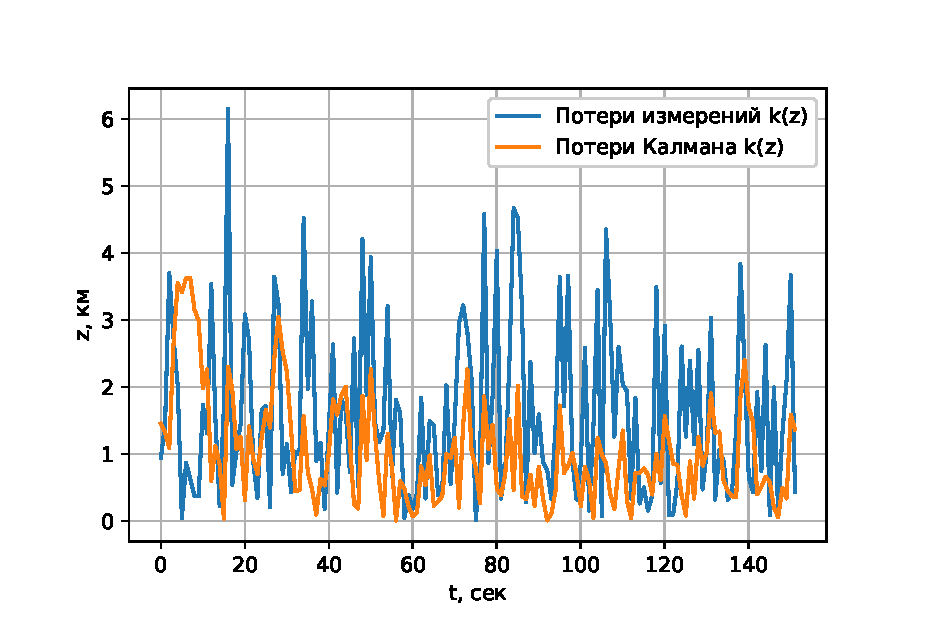
\includegraphics[width=1\linewidth]{images/kalmanz.eps} \\ а)}
\end{minipage}
\hfill
\begin{minipage}[h]{0.49\linewidth}
\center{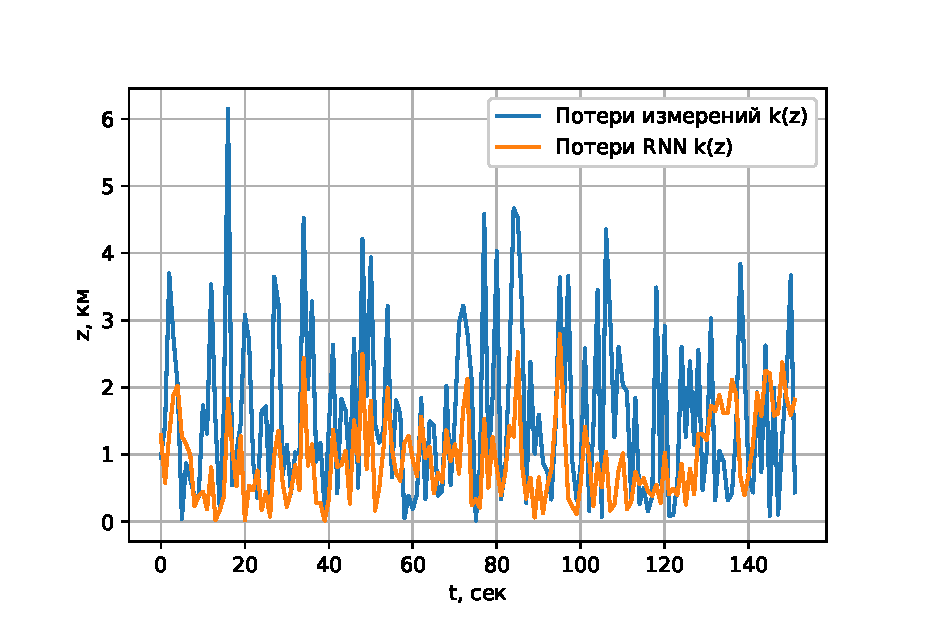
\includegraphics[width=1\linewidth]{images/nnz.eps} \\ б)}
\end{minipage}
\caption{Графики ошибки по оси $z$. а) для классического фильтра Калмана; б) для фильтра Калмана с NN.}
\label{batlz}
\end{figure}

Из графиков видно, что ошибка фильтрации алгоритмом Калмана с нейронной сетью ниже, чем у классического.  Но из-за неверных предсказаний о первой координате, неточность у фильтра с NN в начале может быть выше, чем у стандартного фильтра.

Качественно рассмотрим графики проекций траектории на плоскости $XY$, $XZ$, $YZ$:

\begin{figure}[h!]
\begin{center}
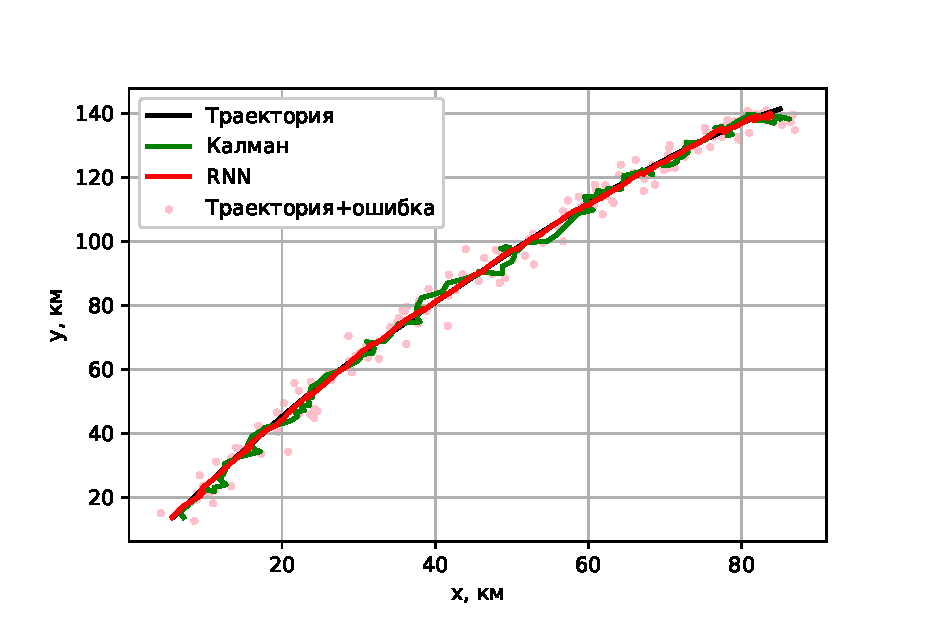
\includegraphics[width=0.7\textwidth]{images/xy.eps}
\end{center}
\caption{Средняя точность по траекториям} \label{xy}
\end{figure}

\begin{figure}[h!]
\begin{center}
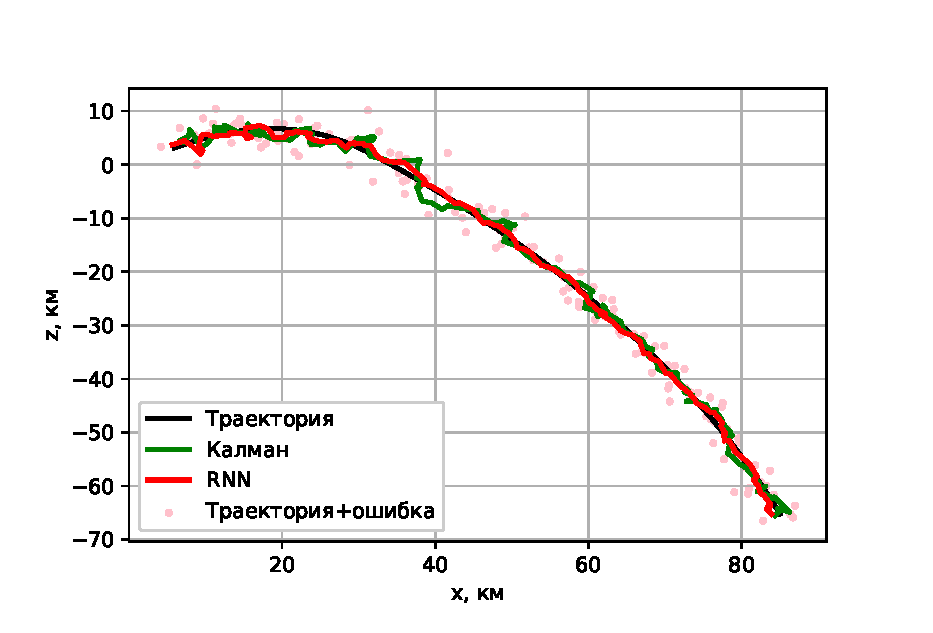
\includegraphics[width=0.7\textwidth]{images/xz.eps}
\end{center}
\caption{Средняя точность по траекториям} \label{xz}
\end{figure}
\newpage
\begin{figure}[h!]
\begin{center}
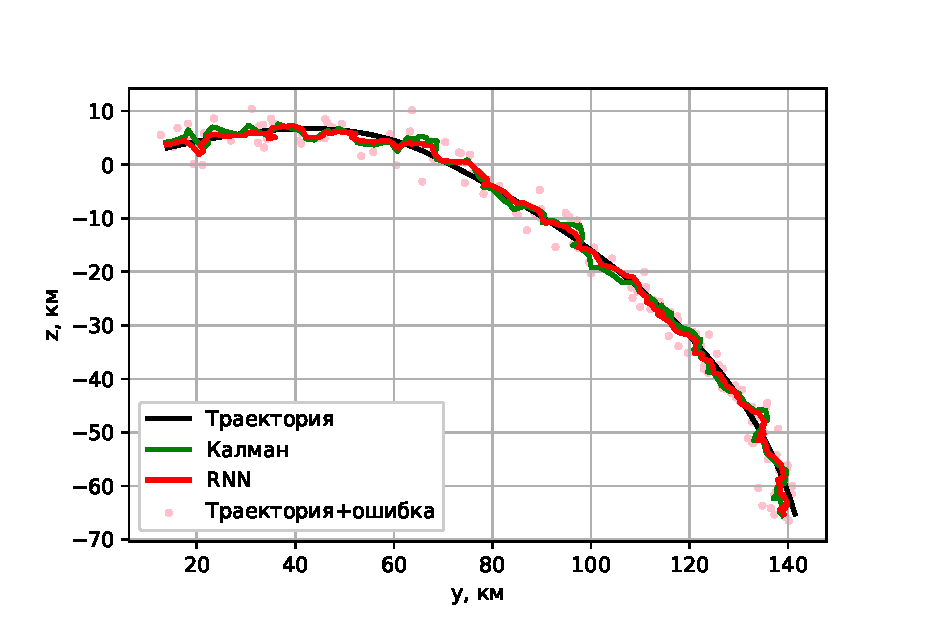
\includegraphics[width=0.7\textwidth]{images/yz.eps}
\end{center}
\caption{Средняя точность по траекториям} \label{yz}
\end{figure}

Оба фильтра хорошо прибежают сигнал к истинному, но фильтр с нейронной сетью, полагаясь на <<память>>,  лучше обрабатывает траекторию,  самостоятельно подстраиваясь под спектор шума.

\newpage
\subsection{Фильтрация траекторий сверхзвуковых измерений}
Смоделируем пример траектории сверхзвукового объекта (рис.  \ref{hgvimg0}). 
\begin{figure}[h!]
\begin{center}
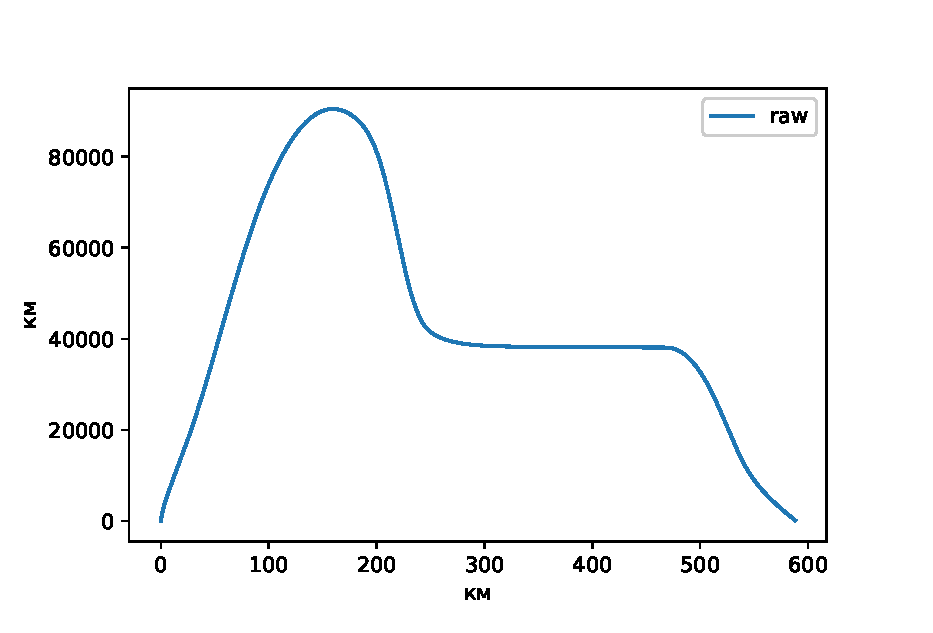
\includegraphics[width=0.6\textwidth]{images/hgv0.eps}
\end{center}
\caption{Смоделированная траектория гиперзвуковой ракеты} \label{hgvimg0}
\end{figure}

Перед анализом набора различных траекторий изменим(улучшим) предварительную обработку данных.  Новыми задачами обработки будут служить:
\begin{enumerate}
\item Смещение траекторий в начальную точку с нулевыми координатами;
\item Отражение траекторий в положительную плоскость;
\item Поворот координат для совмещения начальных траекторий;
\item Нормирование координат.
\end{enumerate}

Данный вид обработки траекторий позволил улучшить фильтрацию данных и минимизировать ошибку отклонения,  сделав её меньше чем у результатов после фильтрации классическим фильтром Калмана (см. гл.  \hyperref[trainval3]{"Сравнение результатов фильтраций"}).

\subsubsection{Обучение и проверка точности}\label{trainval2}
Процесс обучения и валидации аналогичен, как для баллистических объектов (см. гл.  \hyperref[trainval]{"Обучение и проверка точности"} для баллистических траекторий). Приведём характерные для обучения графики ошибки и валидации в зависимости  от эпох:
\begin{figure}[h]
\begin{minipage}[h]{0.49\linewidth}
\center{\includegraphics[width=1\linewidth]{images/losstrain0.eps} \\ а)}
\end{minipage}
\hfill
\begin{minipage}[h]{0.49\linewidth}
\center{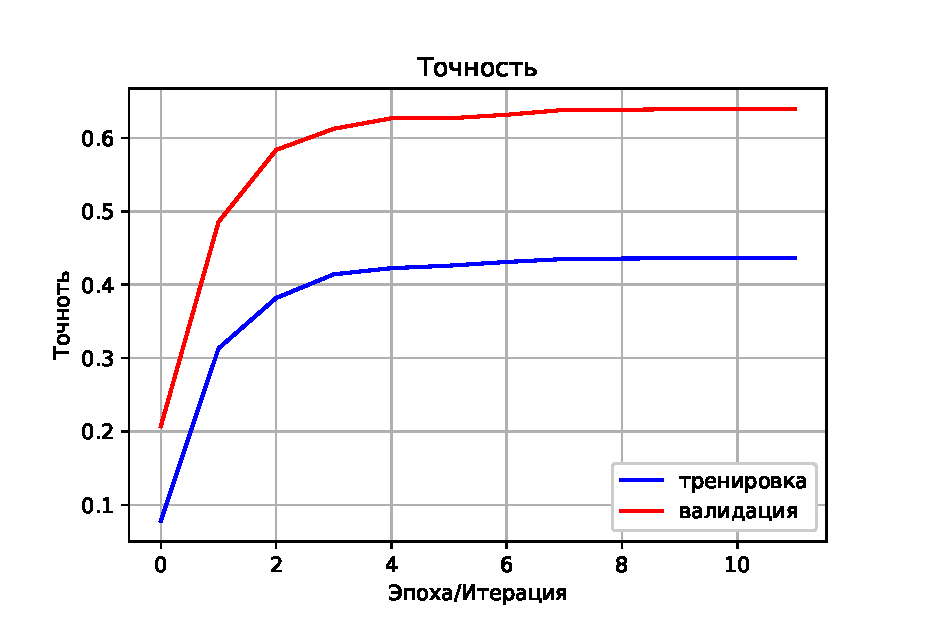
\includegraphics[width=1\linewidth]{images/valtrain0.eps} \\ б)}
\end{minipage}
\caption{Процесс обучения и валидации; а) график зависимости средней по данным MSE ошибки от эпохи; б) график зависимости средней по данным точности от эпохи.}
\label{train0}
\end{figure}

Веса параметров фильтра подбираются методом стохастического градиентного спуска от функции потерь MSE(формула \ref{MSE}):
$$\text{MSE loss: } L(y_t,y_p)=(y_t-y_p)^2.$$

Потери и точность вычисляем по формулам \eqref{loss}, \eqref{accuracy} из главы \hyperref[trainval]{"Обучение и проверка точности"} для траекторий баллистических объектов.

\textbf{Вывод:} Из падения графиков на MSE и росте на Accuracy видно,  что сеть обучается, подтверждая необходимость и верность предварительной обработки траекторий. Точность на валидации чуть выше $63.9\%$, это связано с регуляризацией\footnote{В данном случае говорится об  регуляризация Dropout.} модели и с ложностью поведения траектории. 
\newpage
\subsubsection{Проверка  модели  на контрольных данных}
Приведём процесс тестирования в виде графиков:
 \begin{figure}[h]
\begin{minipage}[h]{0.49\linewidth}
\center{\includegraphics[width=1\linewidth]{images/losstest0.eps} \\ а)}
\end{minipage}
\hfill
\begin{minipage}[h]{0.49\linewidth}
\center{\includegraphics[width=1\linewidth]{images/valtest0.eps} \\ б)}
\end{minipage}
\caption{Процесс тестирования. а) график зависимости средней по данным MSE ошибки от эпохи; б) график зависимости средней по данным точности от эпохи.}
\label{test0}
\end{figure}

Ошибка в среднем $1,2$ по траекториям.  А точности $5\%$ среднем мы достигаем в $68\%$  фильтрации.

\textbf{Вывод:} Сеть успешно обучилась на предварительно обработанных данных,  но возможен рост характеристик точности при  увеличении  обучающей выборки и количества весовых параметров.
\newpage
\subsubsection{Сравнение результатов фильтрации}\label{trainval3}
Сравним результаты фильтраций траекторий полетов сверхзвуковых объектов, уже привычными,  функциями \eqref{loss}, \eqref{accuracy} (из главы \hyperref[trainval2]{"Обучение и проверка точности"} для траекторий баллистических объектов.) обученным фильтром и уже имеющимся фильтром Калмана, представленным в главе \hyperref[kalman1]{"Модель фильтра Калмана"}. Формулы сравнения алгоритмов:
$$
loss = \sqrt{\frac1S{\sum{(\mathbf{\widehat{x}}-\mathbf{x_\text{real}})^2}}},
$$
$$
accuracy =  \frac1S{\sum{\left(\frac{| \mathbf{\widehat{x}}-\mathbf{x_\text{real}}|}{\mathbf{x_\text{real}}}\leqslant D\right)}},
$$
где $\mathbf{\widehat{x}}$ -- вектор оценочных значений  фазового вектора, $\mathbf{x_\text{real}}$-- действительный фазовый вектор,  $D = 0,05$ -- допустимая ошибка $5\%$, $S$ --   колличество элементов в фазовом векторе.


\begin{figure}[h!]
\begin{center}
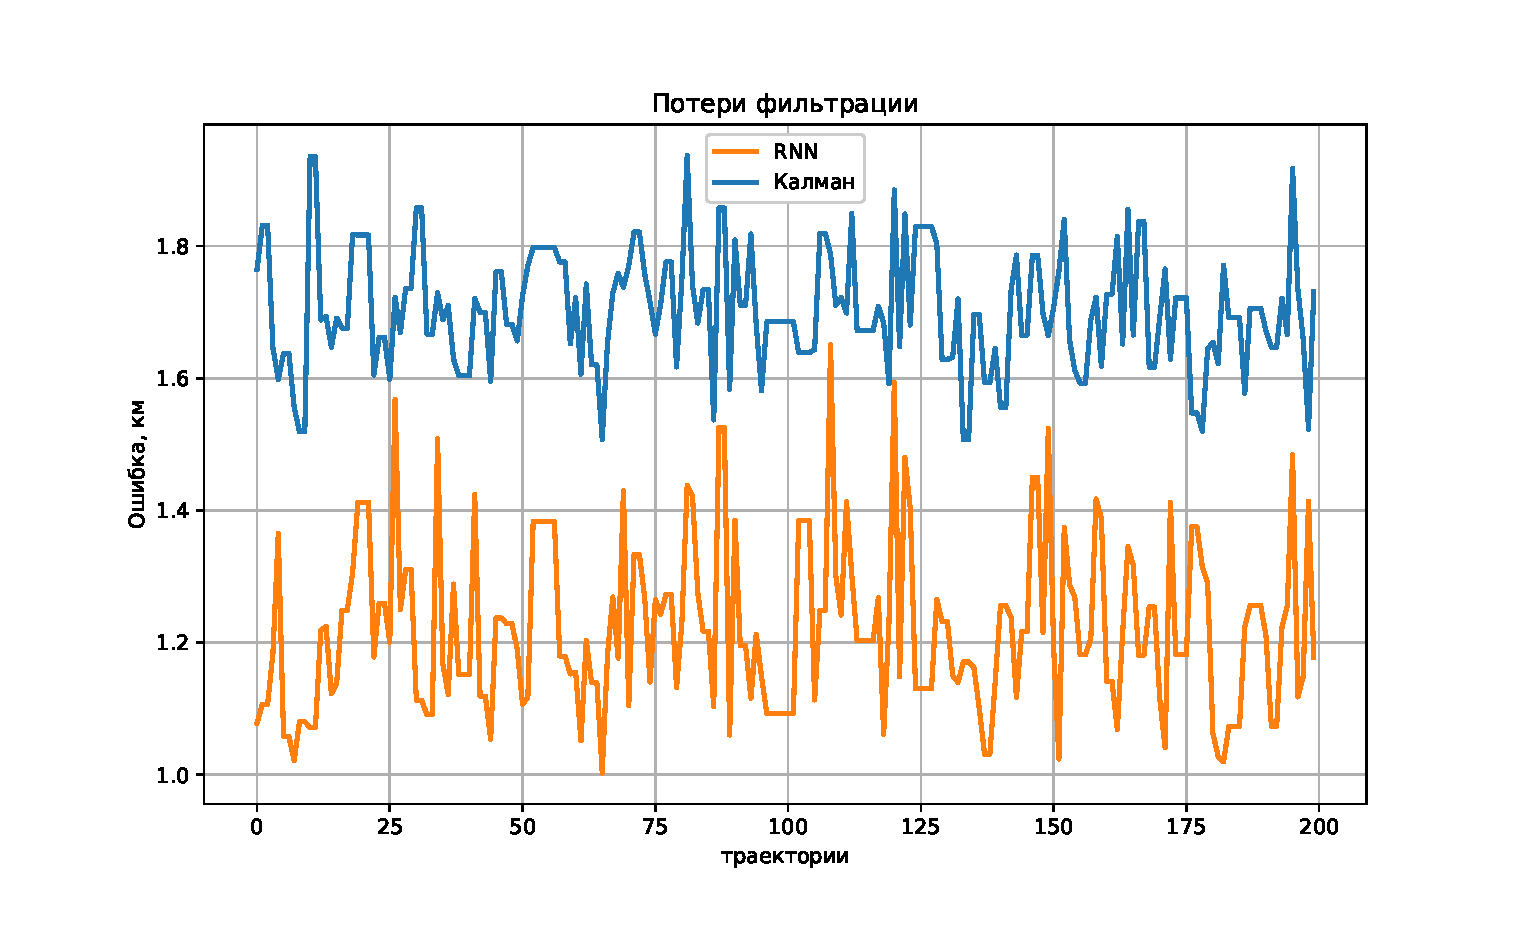
\includegraphics[width=0.6\textwidth]{images/battle3.eps}
\end{center}
\caption{Средние MSE потери по траекториям} \label{battle3}
\end{figure}


\begin{figure}[h!]
\begin{center}
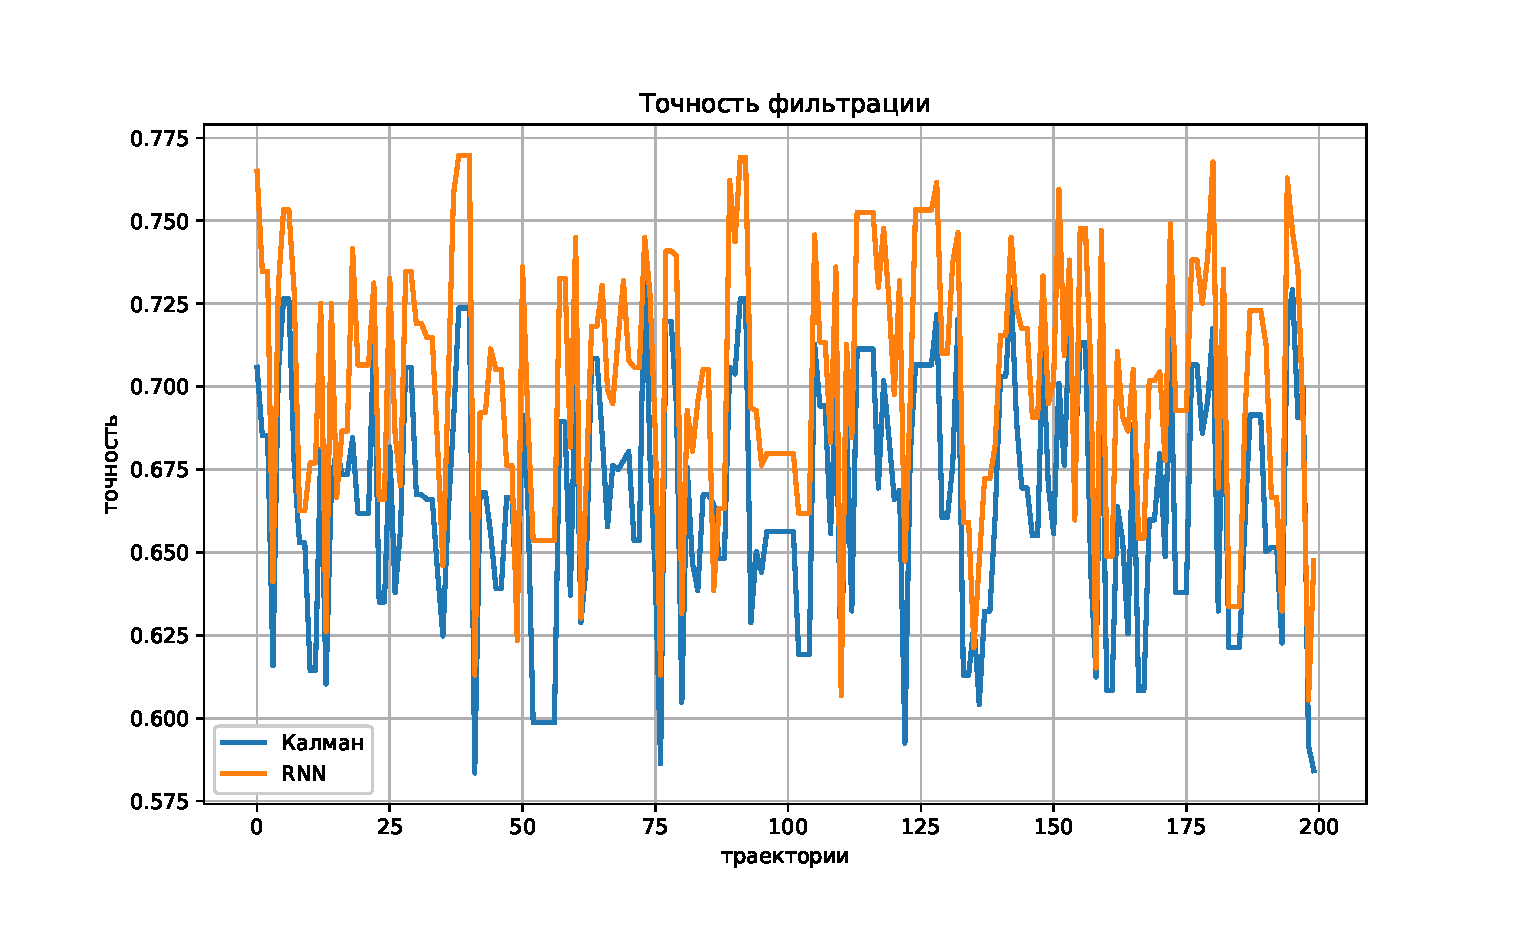
\includegraphics[width=0.6\textwidth]{images/battle4.eps}
\end{center}
\caption{Средняя точность по траекториям} \label{battle4}
\end{figure}

Средние по траекториям потери RNN фильтра Калмана составляют $0.8$ км,  тогда как у классического девяти-мерного фильтра они равны $1.7$ км.

В $5\%$-ую точность в среднем по траектории попадают $72\%$ результатов фильтрации RNN,  и $66\%$ для фильтра Калмана. 

Для исследования характеристик  фильтров, также рассмотрим их работу не в среднем, а на конкретной произвольной траектории.  Будем выводить графики вида: |<<сигнал>>-<<сигнал+шум>>| и рядом |<<фильтрованный сигнал>>-<<сигнал+шум>>| в зависимости от времени.

 \begin{figure}[h]
\begin{minipage}[h]{0.49\linewidth}
\center{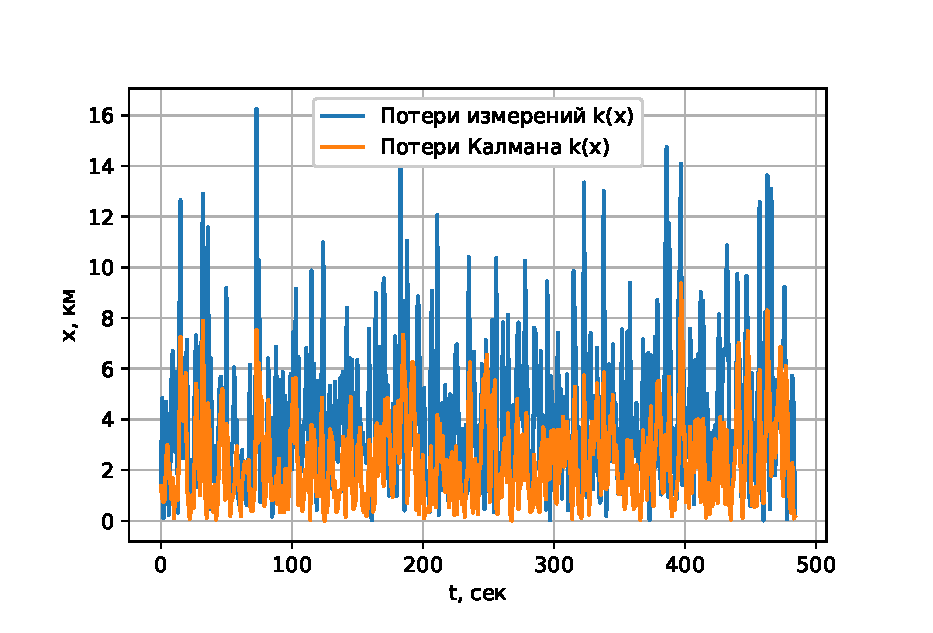
\includegraphics[width=1\linewidth]{images/kalmanx0.eps} \\ а)}
\end{minipage}
\hfill
\begin{minipage}[h]{0.49\linewidth}
\center{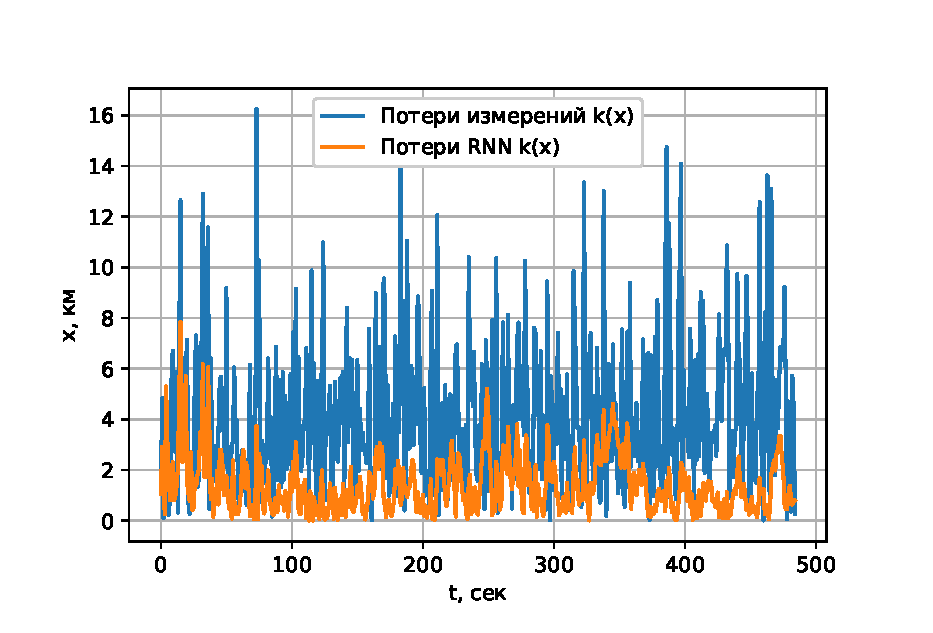
\includegraphics[width=1\linewidth]{images/nnx0.eps} \\ б)}
\end{minipage}
\caption{Графики ошибки по оси $x$. а) для классического фильтра Калмана; б) для фильтра Калмана с NN.}
\label{batlx0}
\end{figure}

 \begin{figure}[h]
\begin{minipage}[h]{0.49\linewidth}
\center{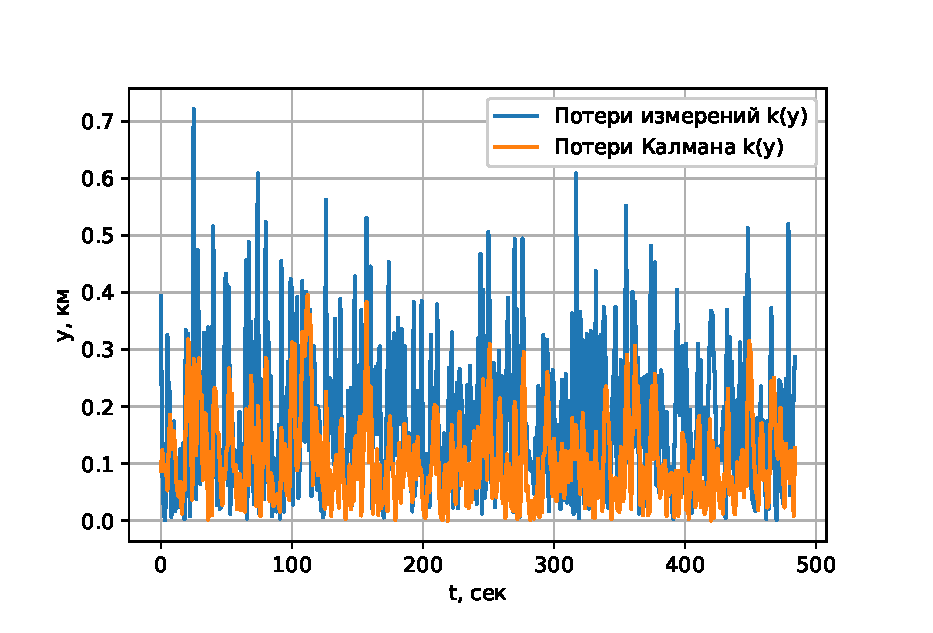
\includegraphics[width=1\linewidth]{images/kalmany0.eps} \\ а)}
\end{minipage}
\hfill
\begin{minipage}[h]{0.49\linewidth}
\center{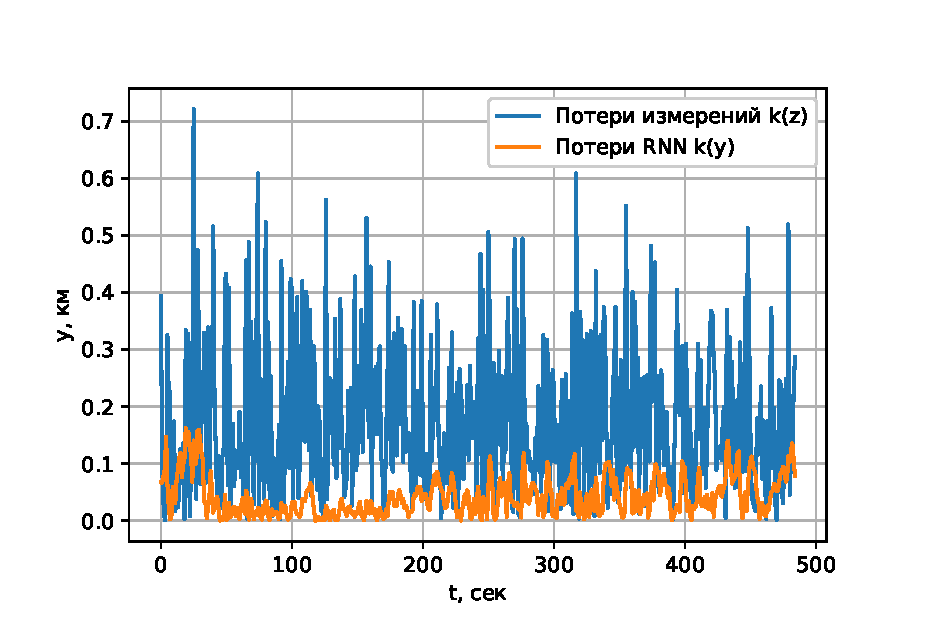
\includegraphics[width=1\linewidth]{images/nny0.eps} \\ б)}
\end{minipage}
\caption{Графики ошибки по оси $y$. а) для классического фильтра Калмана; б) для фильтра Калмана с NN.}
\label{batly0}
\end{figure}

\newpage

 \begin{figure}[h]
\begin{minipage}[h]{0.49\linewidth}
\center{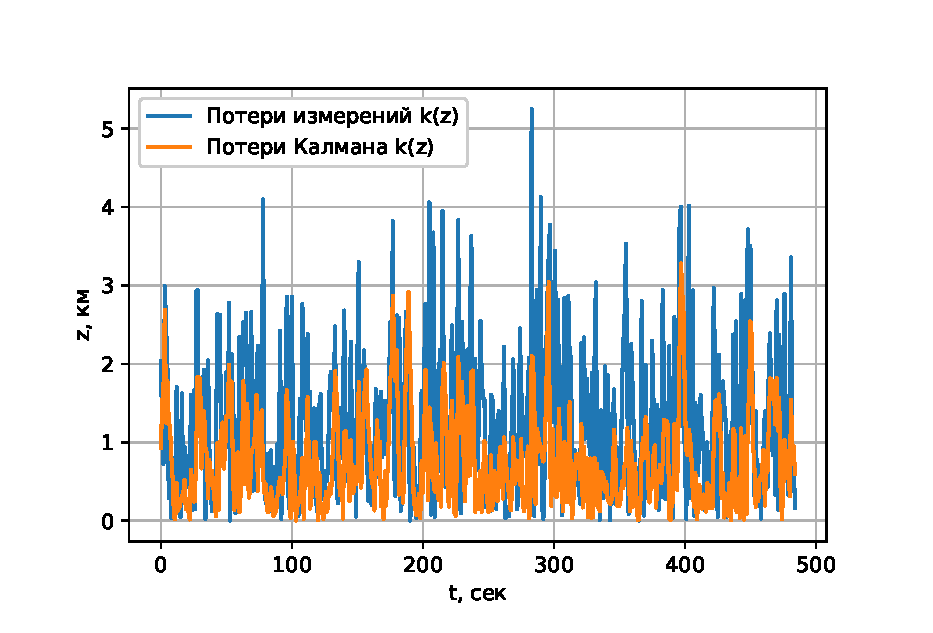
\includegraphics[width=1\linewidth]{images/kalmanz0.eps} \\ а)}
\end{minipage}
\hfill
\begin{minipage}[h]{0.49\linewidth}
\center{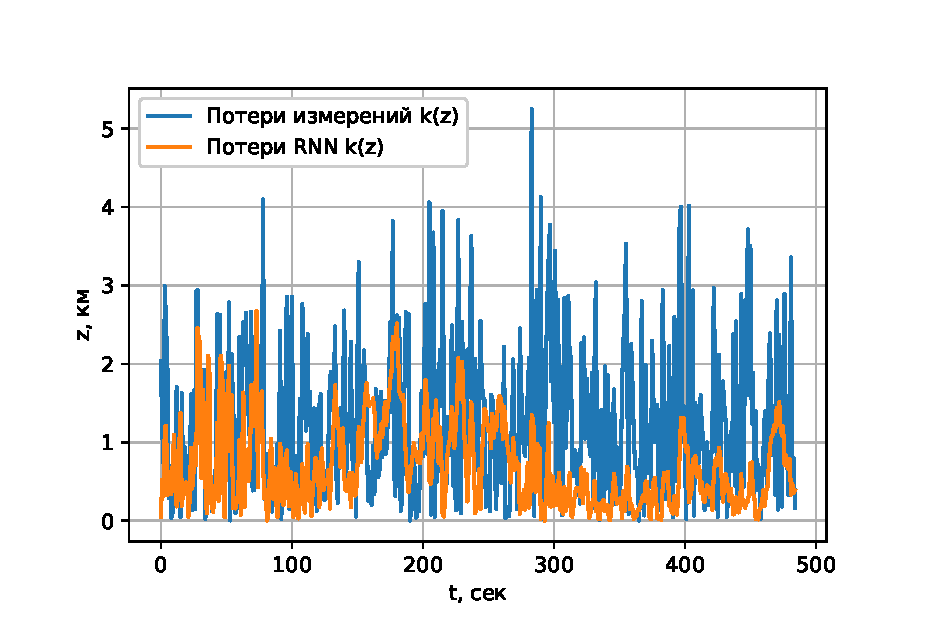
\includegraphics[width=1\linewidth]{images/nnz0.eps} \\ б)}
\end{minipage}
\caption{Графики ошибки по оси $z$. а) для классического фильтра Калмана; б) для фильтра Калмана с NN.}
\label{batlz0}
\end{figure}
Из графиков видно, что ошибка фильтрации алгоритмом Калмана с нейронной сетью ниже, чем у классического.  Но из-за неверных предсказаний о первой координате, неточность у фильтра с NN в начале может быть выше, чем у стандартного фильтра.

Качественно рассмотрим графики проекций траектории на плоскости $XY$, $XZ$, $YZ$:

\begin{figure}[h!]
\begin{center}
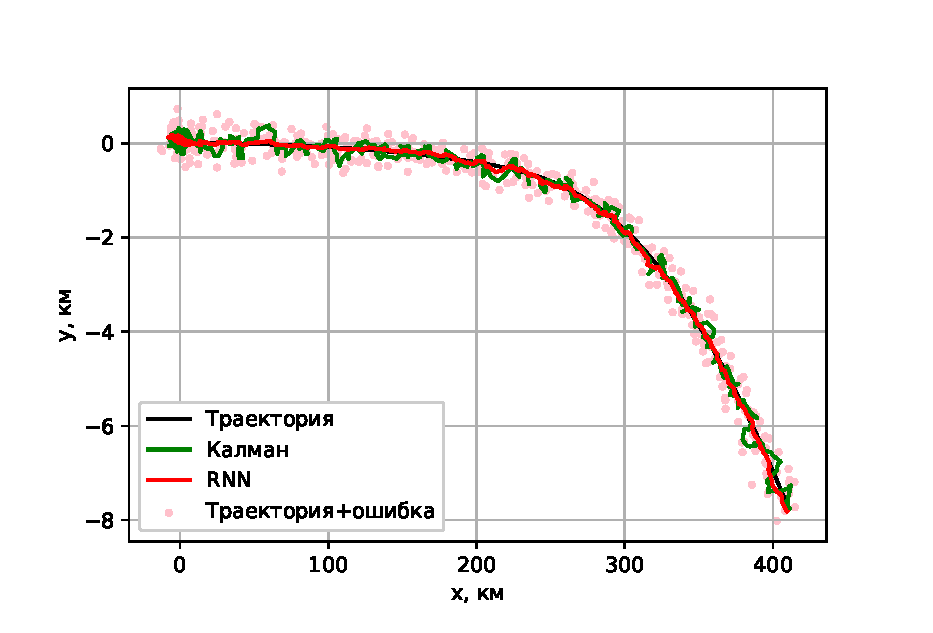
\includegraphics[width=0.7\textwidth]{images/xy0.eps}
\end{center}
\caption{Средняя точность по траекториям} \label{xy0}
\end{figure}

\begin{figure}[h!]
\begin{center}
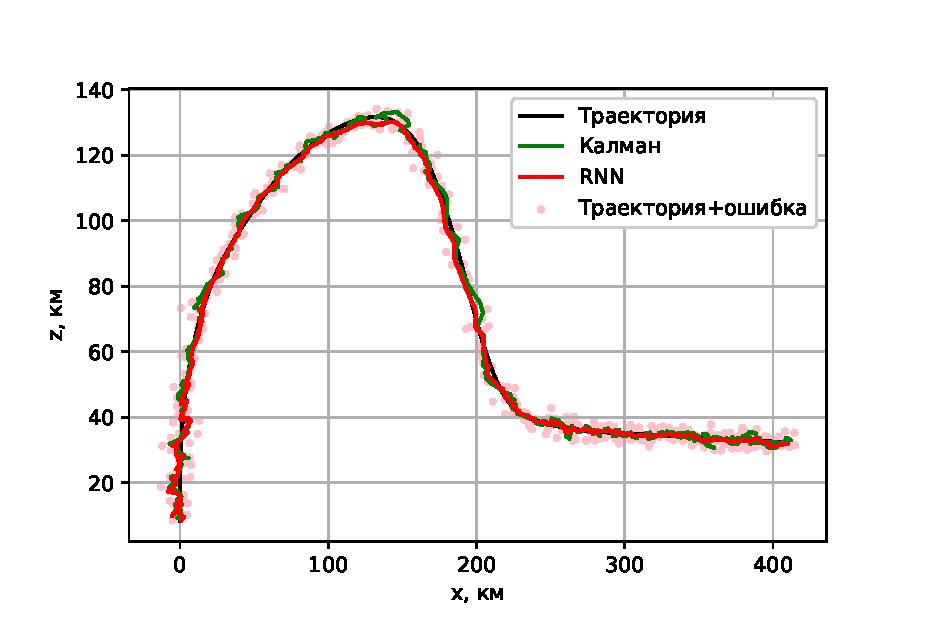
\includegraphics[width=0.7\textwidth]{images/xz0.eps}
\end{center}
\caption{Средняя точность по траекториям} \label{xz0}
\end{figure}
\newpage
\begin{figure}[h!]
\begin{center}
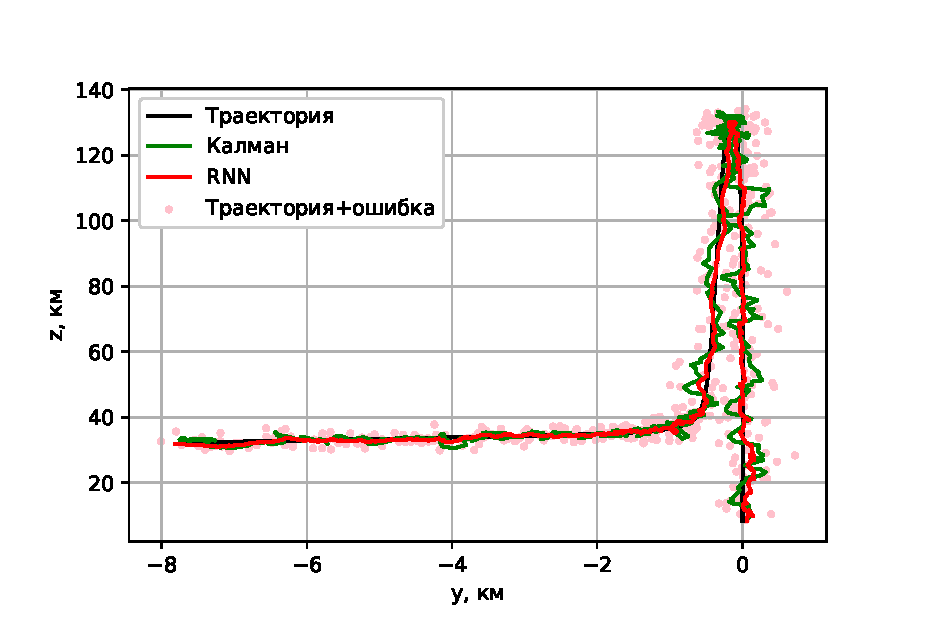
\includegraphics[width=0.7\textwidth]{images/yz0.eps}
\end{center}
\caption{Средняя точность по траекториям} \label{yz0}
\end{figure}

Фильтр с нейронной сетью имеет существенно более низкую ошибку определения траектории движения за счет эффекта памяти при обучении.

\newpage
\section{Выводы}

\begin{itemize}
\item Исследовали и реализовали модель классического алгоритма  Калмана;
\item Изучили вопросы и проблемы связанные с фильтрацией,   нашли решение в применение нейронных сетей к фильтру;
\item Разработали систему фильтрации траекторий движения объектов рекуррентной нейронной сетью(LSTM) с уравнением экстраполяции Калмана;
\item Сравнили результаты двух моделей фильтров: 
\begin{itemize}
\item Средняя квадратичная ошибка по траекториям баллистических объектов для фильтра на нейронной сети составляют $0,9$ км,  у классического девяти-мерного фильтра они равны $1,2$ км;
\item В $5\%$-ую точность в среднем по траектории баллистических объектов попадают $81\%$ результатов фильтрации RNN,  и $73\%$ для фильтра Калмана;
\item Средние по траекториям сверхзвуковых объектов потери RNN фильтра Калмана составляют $0.8$ км,  у классического девяти-мерного фильтра они равны $1,7$ км;
\item В $5\%$-ую точность в среднем по траектории сверхзвуковых объектов попадают $72\%$ результатов фильтрации RNN,  и $66\%$ для фильтра Калмана;
\end{itemize}
\end{itemize}

Данный метод фильтрации может найти свое применение и реализацию во многих сферах, связанных с обработкой фазовых векторов.  Также работа в перспективе может иметь ряд улучшений связанных со снижением ошибки определения траектории и с фильтраций траекторий иных физических объектов.  Исследование предполагает более глубокое изучение и сравнение других отличительных характеристик фильтров.   

В планах на дальнейшее развитие - продолжение разработки затронутой в дипломе темы, а именно:
\begin{itemize}
\item Улучшение архитектуры нейронной сети для уменьшения ошибки определения траектории;
\item Реализация программного обеспечения для тестирования фильтра в полевых условиях на полигоне;
\item Проведение более детального исследования по сравнению иных характерных качеств моделей фильтров.
\end{itemize}
\newpage
\section{Список литературы}
\renewcommand{\refname}{ }

	%\linenumbers
	\bibliographystyle{unsrt}
	\bibliography{thesis.bib}
	\begin{thebibliography}{7}
	\bibitem{KalmanPython} Книга Roger Labbe  \href{https://github.com/rlabbe/Kalman-and-Bayesian-Filters-in-Python}{ <<Kalman and Bayesian Filters in Python>>} 2014г;
	\bibitem{KalmanBook} Статья  R. E. KALMAN \href{http://www.cs.unc.edu/~welch/kalman/media/pdf/Kalman1960.pdf}{<<A New Approach to Linear Filtering and Prediction Problems>>} 1960г;
	\bibitem{nnkategor} Дипломная работа Фонарев А. Ю. \href{http://www.machinelearning.ru/wiki/images/9/99/Diploma_fonarev.pdf}{<<Машинное обучение с категориальными признаками.>>} 2014г;
	\bibitem{voron}  Курс лекций К. В. Воронцов \href{http://www.machinelearning.ru/wiki/images/6/6d/Voron-ML-1.pdf}{<<Математические методы обучения по прецедентам (теория обучения машин).>>};
	\bibitem{lasso}Книга Tibshirani, Robert  \href{https://www.researchgate.net/publication/228781252_Regression_shrinkage_and_selection_via_the_elastic_net_with_applications_to_microarrays}{<<Regression Shrinkage and Selection via the lasso>>} 1996г;
	\bibitem{Spokbook}Книга Spokoiny, Vladimir, Dickhaus, Thorsten <<Basics of Modern Mathematical Statistics>> 2015г;
	\bibitem{mtrixgrad}Методическое  пособие по вычислению матричных производных Justin Johnson <<Derivatives, Backpropagation, and Vectorization>> 2017г;
	\bibitem{ReLearning}Книга Richard S. Sutton and Andrew G. Barto <<Reinforcement Learning: An Introduction second edition>> 2018г;
	\bibitem{NN} Курс по машинному обучению МФТИ(НИУ)  \href{https://github.com/girafe-ai/ml-mipt}{<<Курс по машинному обучению.>> } 2014г;
	\bibitem{RNN} Лекция  7  \href{https://web.stanford.edu/class/cs224n/slides/cs224n-2019-lecture07-fancy-rnn.pdf}{<<Natural Language Processing with Deep Learning CS224N/ Ling28.>> } 2019г;
	\bibitem{neural_Kalman_filter} Документ конференции International Conference on Neural Networks; M.W. Owen, S.C. Stubberud \href{http://ieeexplore.ieee.org/document/833522/}{<<Interacting multiple model tracking using a neural extended Kalman filter.>> } 1999г;
	\bibitem{ConvolutionalSequence} Статья из рецензируемого журнала Jonas Gehring, Michael Auli, David Grangier, Denis Yarats, Yann N. Dauphin \href{https://arxiv.org/abs/1705.03122}{ <<Convolutional Sequence to Sequence Learning>>} 2017г;
	\bibitem{Convolutional_NN} Статья из рецензируемого журнала Anastasia Borovykh, Sander Bohte, Cornelis W. Oosterlee  \href{https://arxiv.org/abs/1703.04691}{ <<Conditional Time Series Forecasting with Convolutional Neural Networks
>>} 2018г;
	\bibitem{Convolutional_NN_Trajectory} Книга Nishant Nikhil, Brendan Tran Morris  \href{https://link.springer.com/chapter/10.1007%2F978-3-030-11015-4_16}{ <<Convolutional Neural Network for Trajectory Prediction>>} 2019г;
	\end{thebibliography}
\end{document}
